\documentclass[11pt,a4paper]{article}

%==================== PACKAGES ====================
\usepackage[utf8]{inputenc}
\usepackage[T1]{fontenc}
\usepackage{lmodern}
\usepackage[french]{babel}
\usepackage[top=2.3cm,bottom=2.3cm,left=2.3cm,right=2.3cm]{geometry}
\usepackage{microtype}
\usepackage{graphicx}
\usepackage{xcolor}
\usepackage{float}
\usepackage[section]{placeins}
\usepackage{amsmath,amssymb}
\usepackage{booktabs}
\usepackage{array}
\usepackage{listings}
\usepackage{caption}
\usepackage{subcaption}
\usepackage{etoolbox}
\usepackage{titlesec}
\usepackage{fancyhdr}
\usepackage{enumitem}
\usepackage[most]{tcolorbox}
\usepackage[colorlinks=true,linkcolor=mainblue,citecolor=mainblue,urlcolor=mainblue]{hyperref}

\hypersetup{pdftitle={TP2 TNS -- Débruitage par filtre de Wiener},
            pdfauthor={Jebali Fares, Rebah Idriss}}

% Les figures peuvent être dans figs/ ou dans le dossier courant
\graphicspath{{figs/}{./}}

%==================== COULEURS ====================
\definecolor{mainblue}{RGB}{0,70,140}
\definecolor{lightblue}{RGB}{50,110,180}
\definecolor{codebg}{RGB}{245,248,252}
\definecolor{codegreen}{RGB}{0,128,0}
\definecolor{codepurple}{RGB}{140,30,160}
\definecolor{resgreen}{RGB}{0,120,70}

%==================== TITRES ====================
\titleformat{\section}
  {\huge\bfseries\color{mainblue}\raggedright}
  {\thesection}{0.6em}{}
  [\vspace{0.2em}{\color{mainblue}\titlerule[1.5pt]}]
\titleformat{\subsection}
  {\Large\bfseries\color{lightblue}}
  {\thesubsection}{0.6em}{}
\titleformat{\subsubsection}
  {\large\bfseries\color{lightblue}}
  {\thesubsubsection}{0.6em}{}
\titlespacing*{\section}{0pt}{0pt}{1.2em}
\titlespacing*{\subsection}{0pt}{1.6em}{0.7em}
\titlespacing*{\subsubsection}{0pt}{1.1em}{0.5em}

% Chaque partie commence sur une nouvelle page
\pretocmd{\section}{\clearpage}{}{}

%==================== EN-TETE ET PIED DE PAGE ====================
\pagestyle{fancy}
\fancyhf{}
\fancyhead[L]{\small\color{mainblue}INSAT -- RT4}
\fancyhead[C]{\small\color{mainblue}Débruitage par filtre de Wiener}
\fancyhead[R]{\small\color{mainblue}TNS -- TP n°2}
\fancyfoot[C]{\small\thepage}
\renewcommand{\headrulewidth}{0.6pt}
\renewcommand{\headrule}{\hbox to\headwidth{\color{mainblue}\leaders\hrule height \headrulewidth\hfill}}
\setlength{\headheight}{15pt}

%==================== LEGENDES ====================
\captionsetup{font=small,labelfont={bf,color=mainblue},labelsep=period}
\captionsetup[subfigure]{font=small}

%==================== CODE ====================
\lstdefinestyle{matlabstyle}{
  language=Matlab,
  basicstyle=\ttfamily\footnotesize,
  columns=flexible,
  keepspaces=true,
  keywordstyle=\color{blue}\bfseries,
  commentstyle=\color{codegreen}\itshape,
  stringstyle=\color{codepurple},
  backgroundcolor=\color{codebg},
  frame=single,
  rulecolor=\color{mainblue},
  breaklines=true,
  showstringspaces=false,
  numbers=left,
  numberstyle=\tiny\color{gray},
  xleftmargin=1.5em,
  framexleftmargin=1.5em,
  aboveskip=0.8em,
  belowskip=0.8em
}
\lstset{style=matlabstyle}

%==================== ENCADRES ====================
% Enoncé de la question
\newtcolorbox{enonce}{
  enhanced, breakable,
  colback=gray!6, colframe=gray!45,
  boxrule=0.5pt, arc=2mm,
  left=6pt, right=6pt, top=3pt, bottom=3pt
}
% Réponse chiffrée / conclusion directe
\newtcolorbox{resultat}[1][Résultat]{
  enhanced, breakable,
  colback=resgreen!6, colframe=resgreen,
  coltitle=white, fonttitle=\bfseries,
  title=#1, arc=2mm, boxrule=0.8pt,
  left=6pt, right=6pt, top=4pt, bottom=4pt
}
% Interprétation
\newtcolorbox{interpretation}[1][Interprétation]{
  enhanced, breakable,
  colback=mainblue!5, colframe=mainblue,
  coltitle=white, fonttitle=\bfseries,
  title=#1, arc=2mm, boxrule=0.8pt,
  left=6pt, right=6pt, top=4pt, bottom=4pt
}

\setlist[itemize]{label=\color{mainblue}\textbullet, itemsep=2pt, topsep=3pt}
\setlist[enumerate]{itemsep=2pt, topsep=3pt}

\begin{document}

%==================== PAGE DE GARDE ====================
\begin{titlepage}
    \thispagestyle{empty}
    \centering

    
\includegraphics[height=2.5cm]{logo.jpg}
    \hfill
    
\includegraphics[height=2.5cm]{logo_carthage.jpg}

    \vspace{0.5cm}
    {\small Année universitaire : 2026/2027}

    \vfill

    {\color{mainblue}\rule{\linewidth}{1.5pt}}\\[0.6cm]
    {\Huge\bfseries\color{mainblue} Compte rendu de\\[0.3cm] Traitement Numérique du Signal}\\[0.6cm]
    {\color{mainblue}\rule{\linewidth}{1.5pt}}

    \vspace{1.5cm}
    {\LARGE\bfseries TP n°2}\\[0.4cm]
    {\large Débruitage par filtre de Wiener}

    \vfill

    \underline{Filière :} \textbf{RT4} \hspace{2cm} \underline{Groupe :} \textbf{1}

    \vspace{1.5cm}

    \underline{Réalisé par :}\\[0.4cm]
    \textbf{Jebali Fares}\\[0.2cm]
    \textbf{Rebah Idriss}

    \vspace{1cm}
    {\small Responsable Cours/TD/TP : R. Amara Boujemâa}

    \vfill
\end{titlepage}

%==================== SOMMAIRE ====================
\pagenumbering{roman}
\tableofcontents
\clearpage
\pagenumbering{arabic}

%==================== PARTIE 1 ====================
\section{Partie 1 : Norbert Wiener et Bernard Widrow}

\subsection{Norbert Wiener (1894--1964)}

\begin{enonce}
\textbf{Énoncé :} Quel est son domaine d'expertise ? Sur quelle problématique a-t-il travaillé ? Quelles sont ses principales réalisations ? Quelle est sa position quant à la cybernétique, sous l'angle de l'organisation de systèmes en interaction, en particulier des systèmes auto-régulés ?
\end{enonce}

\textbf{Domaine d'expertise.} Mathématicien américain, professeur au MIT à partir de 1919. Il a travaillé sur l'analyse harmonique, les processus aléatoires, la prédiction et le filtrage des signaux, et la théorie de la commande et de la communication \cite{ethw_wiener}.

\textbf{Problématique.} Pendant la Seconde Guerre mondiale : prédire la position future d'un avion à partir de mesures radar bruitées, pour pointer automatiquement les canons antiaériens. Plus généralement : \emph{comment estimer au mieux un signal utile noyé dans du bruit ?} Ce travail mène au filtre qui porte son nom \cite{wiki_wiener}.

\textbf{Principales réalisations.}
\begin{itemize}
  \item Le \textbf{filtre de Wiener} : filtre linéaire minimisant l'erreur quadratique moyenne, publié en 1949 dans \emph{Extrapolation, Interpolation, and Smoothing of Stationary Time Series} \cite{wiener1949}.
  \item Le \textbf{processus de Wiener} (modèle mathématique du mouvement brownien, 1923) et le théorème de \textbf{Wiener--Khinchin}, qui relie autocorrélation et densité spectrale de puissance \cite{ethw_wiener}.
  \item La \textbf{cybernétique}, fondée avec son livre \emph{Cybernetics: or Control and Communication in the Animal and the Machine} (1948) \cite{wiener1948}.
\end{itemize}

\textbf{Position sur la cybernétique.} Le mot vient du grec \emph{kubernêtês}, le timonier \cite{monoskop}. Pour Wiener :
\begin{itemize}
  \item un système (machine, être vivant ou société) est un ensemble d'éléments en interaction qui se comprend par l'\textbf{information} qu'ils échangent, et non par la matière qui le compose ; l'information mesure son degré d'organisation ;
  \item l'\textbf{auto-régulation} repose sur la \textbf{rétroaction négative} : le système mesure l'écart entre son état et son but, puis corrige son action (thermostat, pilote automatique, homéostasie du corps) ;
  \item ces principes sont les mêmes quelle que soit la nature du système : la cybernétique est donc une science transversale du contrôle et de la communication.
\end{itemize}

\subsection{Bernard Widrow (1929--2025)}

\begin{enonce}
\textbf{Énoncé :} Quel est son domaine d'expertise ? Sur quelle problématique a-t-il travaillé ? Quelles sont ses principales réalisations ? Identifier son article qui traite des principaux réseaux de neurones adaptatifs.
\end{enonce}

\textbf{Domaine d'expertise.} Professeur à Stanford, spécialiste du traitement adaptatif du signal et des réseaux de neurones \cite{ethw_widrow}.

\textbf{Problématique.} Le filtre de Wiener exige de connaître les statistiques du signal ($\mathbf{R}_x$, $\mathbf{r}_{dx}$). Widrow cherche un filtre qui \emph{apprend} ses coefficients à partir des données, échantillon par échantillon, en minimisant l'erreur quadratique moyenne.

\textbf{Principales réalisations.}
\begin{itemize}
  \item L'algorithme \textbf{LMS} (\emph{Least Mean Squares}), inventé en 1959 avec son étudiant Ted Hoff \cite{chm_widrow}.
  \item Les réseaux de neurones \textbf{ADALINE} (1960) et \textbf{MADALINE}, entraînés par le LMS \cite{stanford_obit}.
  \item Les applications du filtrage adaptatif : annulation de bruit et d'écho, égalisation, antennes adaptatives \cite{ethw_widrow} ; livre de référence \emph{Adaptive Signal Processing} (1985) \cite{widrowstearns}.
\end{itemize}

\textbf{Article sur les réseaux de neurones adaptatifs.} B.~Widrow et M.~A.~Lehr, « 30 Years of Adaptive Neural Networks: Perceptron, Madaline, and Backpropagation », \emph{Proceedings of the IEEE}, vol.~78, n°~9, pp.~1415--1442, 1990 \cite{widrowlehr1990}.

\subsection{Lien avec le TP}

Le filtre de Wiener du TP calcule directement la solution optimale :
\[
\mathbf{w}_{opt}=\mathbf{R}_x^{-1}\mathbf{r}_{dx},
\qquad
\mathrm{EQM}_{\min}=r_d(0)-\mathbf{w}_{opt}^T\mathbf{r}_{dx},
\]
en estimant $\mathbf{R}_x$ et $\mathbf{r}_{dx}$ par moyennes temporelles (signal supposé stationnaire et ergodique). Le LMS de Widrow converge vers la même solution sans inverser de matrice ni connaître les statistiques :
\[
\mathbf{w}(n+1)=\mathbf{w}(n)+\mu\,e(n)\,\mathbf{x}(n),\qquad e(n)=d(n)-\mathbf{w}^T(n)\mathbf{x}(n).
\]

%==================== PARTIE 2 ====================
\section{Partie 2 : Débruitage d'une harmonique}

On considère $d(n)=\sin(nw_0+\phi)$, $n=1,\dots,N$, avec $N=10^4$, $w_0=0.05\pi$ et $\phi=\pi/4$. Le signal bruité est $x(n)=d(n)+v(n)$, où $v(n)$ est un bruit blanc gaussien $\mathcal{N}(0,\sigma_v^2)$ généré avec \texttt{randn}.

\textbf{Notations.} Le filtre de Wiener d'ordre $P$ estime $d(n)$ à partir du régresseur $\mathbf{x}(n)=[x(n),\,x(n-1),\,\dots,\,x(n-P+1)]^T$ :
\[
\hat d(n)=\mathbf{w}_{opt}^T\mathbf{x}(n),\qquad
\mathbf{w}_{opt}=\mathbf{R}_x^{-1}\mathbf{r}_{dx},\qquad
\mathrm{EQM}_{\min}=r_d(0)-\mathbf{w}_{opt}^T\mathbf{r}_{dx},
\]
où $\mathbf{R}_x$ est la matrice de Toeplitz construite sur $r_x(0),\dots,r_x(P-1)$ et $\mathbf{r}_{dx}=[r_{dx}(0),\dots,r_{dx}(P-1)]^T$. Comme $d$ et $v$ sont indépendants et $v$ centré : $r_x(k)=r_d(k)+\sigma_v^2\,\delta(k)$ et $r_{dx}(k)=r_d(k)$.

\subsection{Question (a) : affichage des signaux}

\begin{enonce}
\textbf{Énoncé :} Afficher une fenêtre de $d(n)$, $x(n)$ et $\hat d(n)$ pour $P=10$ et $\sigma_v^2=0.1$.
\end{enonce}

\textbf{Démarche.}
\begin{enumerate}
  \item Génération de $d(n)$, de $v(n)=\sqrt{\sigma_v^2}\,\texttt{randn}$ et de $x(n)=d(n)+v(n)$.
  \item Estimation de $r_x(k)$ et $r_{dx}(k)=r_d(k)$ par moyennes temporelles (\texttt{xcorr}, retards $0$ à $P-1$).
  \item Construction de $\mathbf{R}_x$ (\texttt{toeplitz}) et résolution de $\mathbf{R}_x\mathbf{w}_{opt}=\mathbf{r}_{dx}$.
  \item Filtrage : $\hat d(n)=\mathbf{w}_{opt}^T\mathbf{x}(n)$ (\texttt{filter}).
\end{enumerate}

\textbf{Code.}
\begin{lstlisting}
clear; clc; close all;

% Parametres
N     = 1e4;          % nombre d'echantillons
n     = (1:N)';
w0    = 0.05*pi;
phi   = pi/4;         % phase fixee
P     = 10;           % ordre du filtre
sigv2 = 0.1;          % variance du bruit

% Signal, bruit, signal bruite
d = sin(n*w0 + phi);
v = sqrt(sigv2)*randn(N,1);
x = d + v;

% Correlations (retards 0 a P-1) : r_dx(k) = r_d(k)
rx = xcorr(x, P-1, 'biased');  rx = rx(P:end);
rd = xcorr(d, P-1, 'biased');  rd = rd(P:end);
Rx = toeplitz(rx);

% Filtre de Wiener et signal debruite
hopt = Rx \ rd;
dhat = filter(hopt, 1, x);

% Affichage d'une fenetre
idx = 101:200;
figure;
plot(idx, d(idx), 'b', idx, x(idx), 'Color', [0.7 0.7 0.7]); hold on;
plot(idx, dhat(idx), 'r', 'LineWidth', 1.5);
grid on; xlabel('n'); ylabel('Amplitude');
legend('d(n)', 'x(n)', 'dhat(n)');
\end{lstlisting}

\begin{figure}[H]
  \centering
  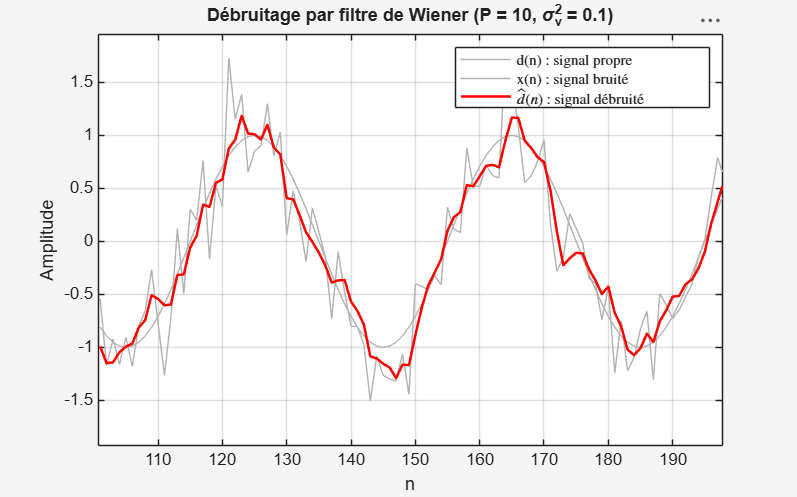
\includegraphics[width=0.9\linewidth]{fig21}
  \caption{Signal propre $d(n)$, signal bruité $x(n)$ et signal débruité $\hat d(n)$ ($P=10$, $\sigma_v^2=0.1$).}
\end{figure}

\begin{interpretation}
\begin{itemize}
  \item RSB avant débruitage : $10\log_{10}(0.5/0.1)\approx 7$~dB ; $x(n)$ fluctue fortement autour de la sinusoïde.
  \item $\hat d(n)$ est beaucoup plus lisse et suit $d(n)$ en phase et en amplitude. Le petit résidu restant est le bruit situé dans la bande passante du filtre, encore large pour $P=10$.
  \item Les $P-1$ premiers échantillons de $\hat d(n)$ sont un régime transitoire : la fenêtre affichée ($n=101$ à $200$) est choisie après cette zone.
\end{itemize}
\end{interpretation}

\subsection{Question (b) : valeur de \texorpdfstring{$\mathrm{EQM}_{\min}$}{EQMmin}}

\begin{enonce}
\textbf{Énoncé :} Déterminer la valeur de $\mathrm{EQM}_{\min}$ en utilisant son expression déduite dans le cours.
\end{enonce}

\textbf{Démarche.} On applique $\mathrm{EQM}_{\min}=r_d(0)-\mathbf{w}_{opt}^T\mathbf{r}_{dx}$, où $r_d(0)$ est la puissance de $d(n)$ (théoriquement $A^2/2=0.5$), soit le premier élément du vecteur \texttt{rd}.

\textbf{Code.} (à la suite du code de la question (a))
\begin{lstlisting}
% EQM_min selon la formule du cours ; rd(1) = r_d(0)
EQM_min = rd(1) - hopt' * rd;
fprintf('EQM_min (P = %d, sigma_v^2 = %.2f) : %.4f\n', P, sigv2, EQM_min);
\end{lstlisting}

\begin{figure}[H]
    \centering
    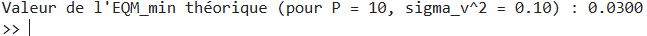
\includegraphics[width=0.85\linewidth]{fig22}
    \caption{Valeur de $\mathrm{EQM}_{\min}$ affichée dans la console ($P=10$, $\sigma_v^2=0.1$).}
\end{figure}

\begin{resultat}
$\mathrm{EQM}_{\min}=0.0300$ pour $P=10$ et $\sigma_v^2=0.1$.
\end{resultat}

\begin{interpretation}
\begin{itemize}
  \item C'est l'erreur minimale atteignable par un filtre RIF d'ordre $10$. Sans filtrage ($\hat d=x$), l'erreur vaut $\sigma_v^2=0.1$ : le filtre la divise par $3.3$, soit un gain de $10\log_{10}(0.1/0.03)\approx 5.2$~dB, cohérent avec le gain mesuré en (f) ($5.4$~dB pour $P=10$).
  \item Avec les corrélations exactes ($r_d(k)=\tfrac12\cos(kw_0)$), on obtient $\mathrm{EQM}_{\min}=0.0279$ : l'écart vient de l'estimation des corrélations sur $N=10^4$ échantillons (voir (d)).
\end{itemize}
\end{interpretation}

\subsection{Question (c) : convergence de \texorpdfstring{$eqm(k)$}{eqm(k)} pour P = 3, 5 et 10}

\begin{enonce}
\textbf{Énoncé :} Afficher l'EQM calculée en ligne $eqm(k)=\frac{1}{k}\sum_{i=1}^{k}(d(i)-\hat d(i))^2$, la stocker dans le vecteur \texttt{eqm} et montrer par simulation qu'elle converge vers $\mathrm{EQM}_{\min}$ pour $P=3$, $5$ et $10$. Afficher les courbes et les droites horizontales d'ordonnée $\mathrm{EQM}_{\min}$. Interpréter.
\end{enonce}

\textbf{Démarche.} Pour chaque $P$ : calcul de $\mathbf{w}_{opt}$, $\hat d(n)$ et $\mathrm{EQM}_{\min}$ ; calcul récursif de $eqm(k)=S_k/k$ avec $S_k=S_{k-1}+(d(k)-\hat d(k))^2$ ; tracé de $eqm(k)$ et de la droite $\mathrm{EQM}_{\min}$ (axe $k$ logarithmique).

\textbf{Code.} (à la suite du code de la question (a))
\begin{lstlisting}
Plist  = [3 5 10];
EQM    = zeros(N, length(Plist));
EQMmin = zeros(1, length(Plist));

for m = 1:length(Plist)
    Pm  = Plist(m);
    rxm = xcorr(x, Pm-1, 'biased'); rxm = rxm(Pm:end);
    rdm = xcorr(d, Pm-1, 'biased'); rdm = rdm(Pm:end);
    hm  = toeplitz(rxm) \ rdm;
    dhm = filter(hm, 1, x);

    S = 0;
    for k = 1:N
        S        = S + (d(k) - dhm(k))^2;
        EQM(k,m) = S / k;
    end
    EQMmin(m) = rdm(1) - hm' * rdm;
    fprintf('P = %2d : EQM_min = %.4f | eqm(N) = %.4f\n', Pm, EQMmin(m), EQM(N,m));
end

% Une figure par P
for m = 1:length(Plist)
    figure;
    plot(1:N, EQM(:,m), 'b', 'LineWidth', 1.3); hold on;
    plot([1 N], [EQMmin(m) EQMmin(m)], 'r--', 'LineWidth', 1.3);
    set(gca, 'XScale', 'log'); grid on;
    ylim([0 3*EQMmin(m)]);
    xlabel('k'); ylabel('eqm(k)');
    title(sprintf('Convergence de eqm(k) vers EQM_{min} (P = %d)', Plist(m)));
    legend('eqm(k)', 'EQM_{min}', 'Location', 'best');
end

% Les trois courbes ensemble
col = lines(3);
figure; hold on;
for m = 1:length(Plist)
    h(m) = plot(1:N, EQM(:,m), 'Color', col(m,:), 'LineWidth', 1.3);
    plot([1 N], [EQMmin(m) EQMmin(m)], '--', 'Color', col(m,:), 'LineWidth', 1);
end
set(gca, 'XScale', 'log'); grid on;
ylim([0 3*max(EQMmin)]);
xlabel('k'); ylabel('eqm(k)');
legend(h, 'P = 3', 'P = 5', 'P = 10', 'Location', 'best');
\end{lstlisting}

\begin{figure}[H]
  \centering
  \begin{subfigure}{0.49\linewidth}
    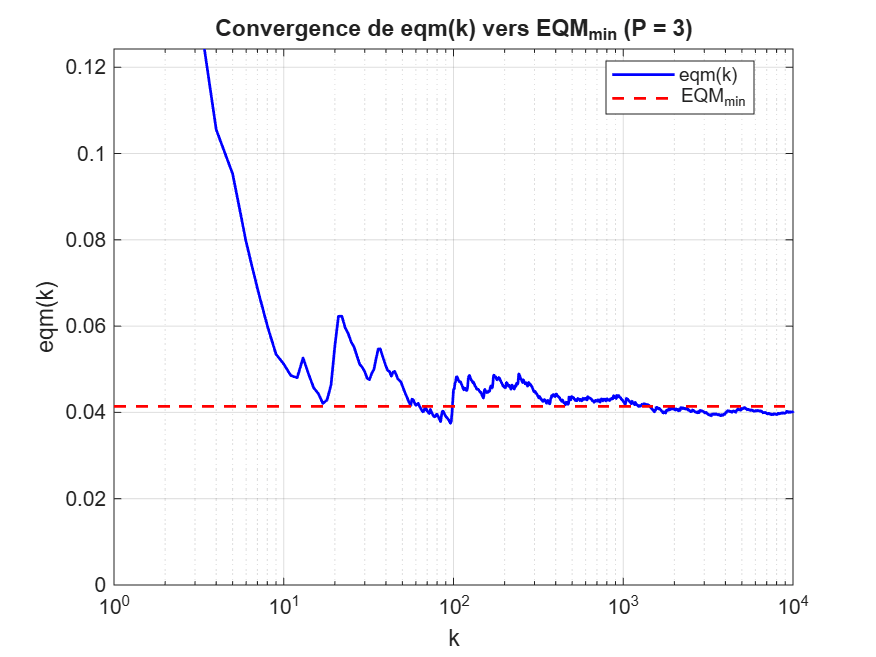
\includegraphics[width=\linewidth]{fig23}
    \caption{$P=3$}
  \end{subfigure}\hfill
  \begin{subfigure}{0.49\linewidth}
    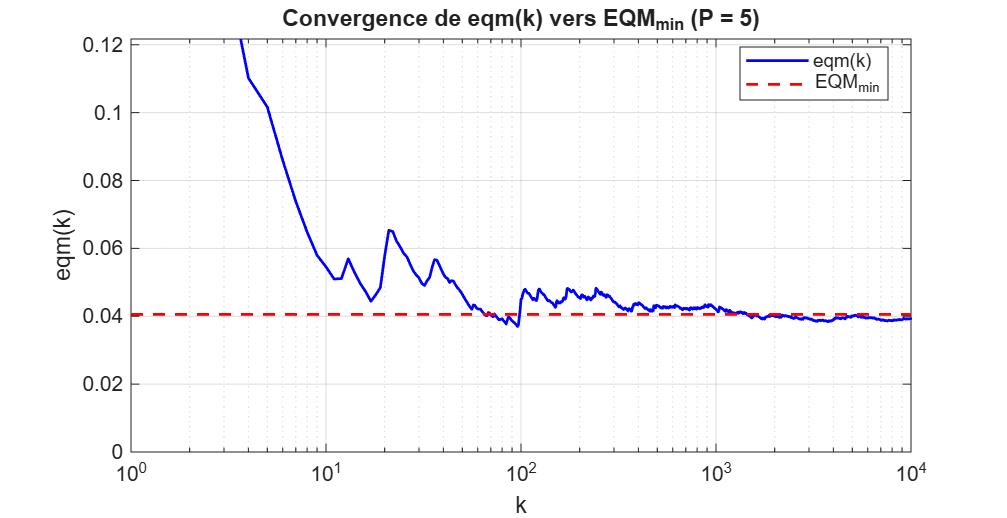
\includegraphics[width=\linewidth]{fig24}
    \caption{$P=5$}
  \end{subfigure}

  \medskip
  \begin{subfigure}{0.49\linewidth}
    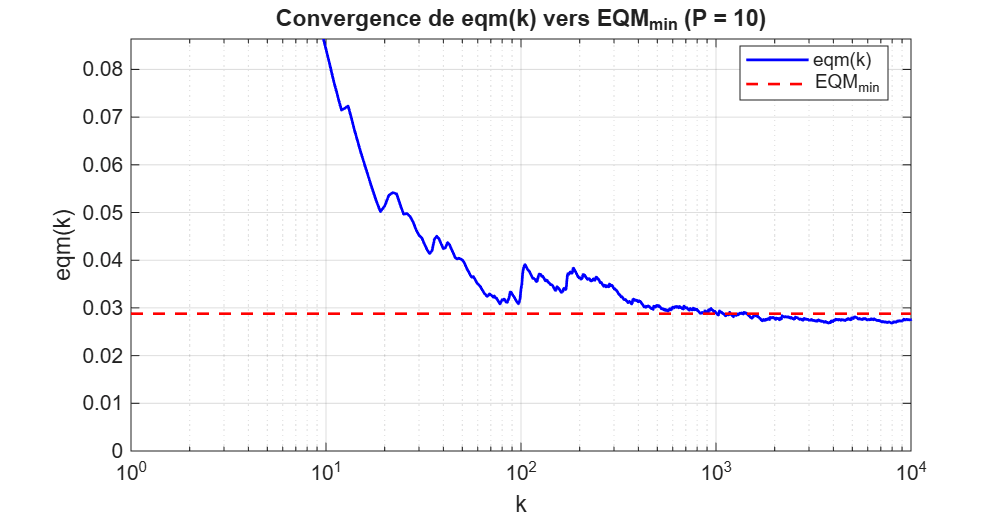
\includegraphics[width=\linewidth]{fig25}
    \caption{$P=10$}
  \end{subfigure}\hfill
  \begin{subfigure}{0.49\linewidth}
    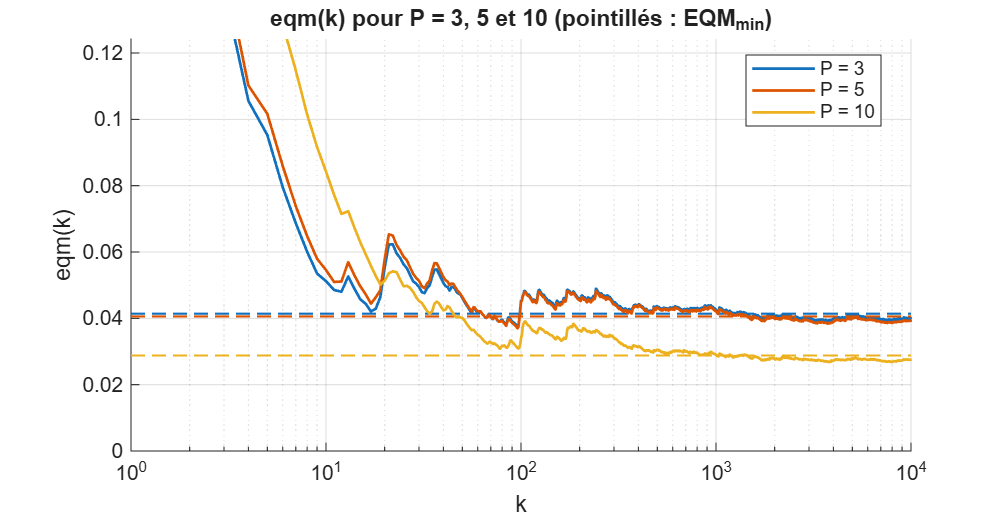
\includegraphics[width=\linewidth]{fig26}
    \caption{Comparaison des trois ordres}
  \end{subfigure}
  \caption{$eqm(k)$ (trait plein) et $\mathrm{EQM}_{\min}$ (pointillés) pour $\sigma_v^2=0.1$.}
\end{figure}

\begin{resultat}
$\mathrm{EQM}_{\min}\approx 0.041$ ($P=3$), $0.040$ ($P=5$) et $0.029$ ($P=10$). Pour chaque ordre, $eqm(k)$ converge vers $\mathrm{EQM}_{\min}$ à environ $10^{-3}$ près à partir de $k\approx 10^3$.\\
{\small (Nouvelle exécution du script, donc nouvelle réalisation du bruit : $0.029$ au lieu de $0.030$ en (b) pour $P=10$.)}
\end{resultat}

\begin{interpretation}
\begin{itemize}
  \item \textbf{Convergence.} La formule du cours donne bien l'erreur réellement obtenue : $eqm(k)$ est une moyenne empirique qui tend vers l'espérance $E[(d-\hat d)^2]=\mathrm{EQM}_{\min}$ (ergodicité).
  \item \textbf{Début des courbes.} L'erreur est élevée au départ à cause du régime transitoire du filtre (les $P-1$ premiers échantillons) et de la moyenne sur peu de points ; le poids de ces valeurs décroît en $1/k$.
  \item \textbf{Écart résiduel} (de l'ordre de $10^{-3}$) : erreur d'estimation des corrélations sur $N=10^4$ échantillons, étudiée en (d).
  \item \textbf{Influence de $P$.} $P=3$ et $P=5$ donnent presque la même erreur ; $P=10$ la réduit nettement : un filtre plus long a une bande passante plus étroite autour de $w_0$ et laisse passer moins de bruit.
\end{itemize}
\end{interpretation}

\subsection{Question (d) : influence de la puissance du bruit}

\begin{enonce}
\textbf{Énoncé :} Tracer la même courbe d'EQM pour $P=10$ et $\sigma_v^2\in\{0.01,\ 0.05,\ 0.1,\ 0.5,\ 1\}$. Interpréter.
\end{enonce}

\textbf{Démarche.} Pour chaque $\sigma_v^2$ : nouveau bruit, calcul de $\mathbf{w}_{opt}$, $\hat d(n)$, $\mathrm{EQM}_{\min}$ et $eqm(k)$ comme en (c). Une figure par valeur, puis une comparaison en échelle log--log. Le script est relancé avec $N=10^5$ pour vérifier l'écart observé à faible bruit.

\textbf{Code.}
\begin{lstlisting}
clear; clc; close all;

% Parametres
N       = 1e4;            % 1e5 pour la verification
n       = (1:N)';
w0      = 0.05*pi;
phi     = pi/4;
P       = 10;
sigList = [0.01 0.05 0.1 0.5 1];
nS      = length(sigList);

d = sin(n*w0 + phi);

EQM    = zeros(N, nS);
EQMmin = zeros(1, nS);

for s = 1:nS
    % Signal bruite pour cette valeur de sigv2
    x = d + sqrt(sigList(s))*randn(N,1);

    % Filtre de Wiener
    rx = xcorr(x, P-1, 'biased'); rx = rx(P:end);
    rd = xcorr(d, P-1, 'biased'); rd = rd(P:end);
    hopt = toeplitz(rx) \ rd;
    dhat = filter(hopt, 1, x);

    % eqm(k) calculee en ligne
    S = 0;
    for k = 1:N
        S        = S + (d(k) - dhat(k))^2;
        EQM(k,s) = S / k;
    end
    EQMmin(s) = rd(1) - hopt' * rd;
    fprintf('sigv2 = %.2f : EQM_min = %.4f | eqm(N) = %.4f\n', ...
            sigList(s), EQMmin(s), EQM(N,s));
end

% Une figure par sigv2
for s = 1:nS
    figure;
    plot(1:N, EQM(:,s), 'b', 'LineWidth', 1.3); hold on;
    plot([1 N], [EQMmin(s) EQMmin(s)], 'r--', 'LineWidth', 1.3);
    set(gca, 'XScale', 'log'); grid on;
    ylim([0 3*EQMmin(s)]);
    xlabel('k'); ylabel('eqm(k)');
    legend('eqm(k)', 'EQM_{min}', 'Location', 'best');
end

% Comparaison (axes log)
col = lines(nS);
figure; hold on;
for s = 1:nS
    h(s) = plot(1:N, EQM(:,s), 'Color', col(s,:), 'LineWidth', 1.3);
    plot([1 N], [EQMmin(s) EQMmin(s)], '--', 'Color', col(s,:));
end
set(gca, 'XScale', 'log', 'YScale', 'log'); grid on;
ylim([0.5*min(EQMmin) 3*max(EQMmin)]);
xlabel('k'); ylabel('eqm(k)');
legend(h, arrayfun(@(v) sprintf('\\sigma_v^2 = %.2f', v), sigList, ...
       'UniformOutput', false), 'Location', 'best');
\end{lstlisting}

\begin{figure}[H]
  \centering
  \begin{subfigure}{0.49\linewidth}
    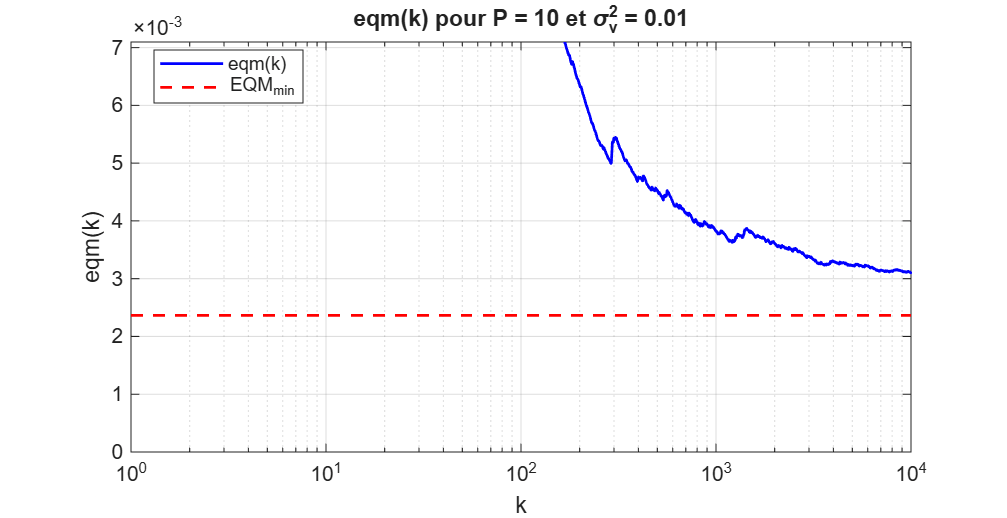
\includegraphics[width=\linewidth]{fig27}
    \caption{$\sigma_v^2=0.01$}
  \end{subfigure}\hfill
  \begin{subfigure}{0.49\linewidth}
    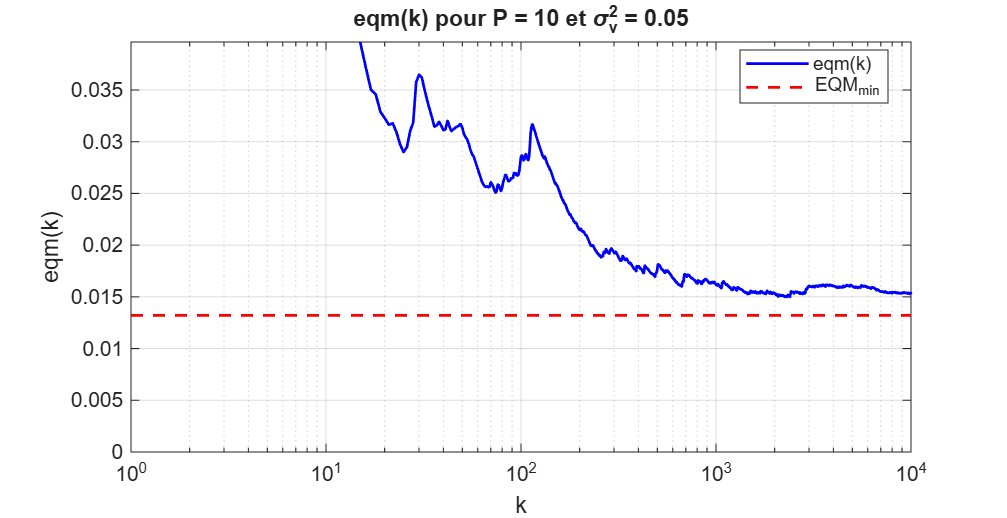
\includegraphics[width=\linewidth]{fig28}
    \caption{$\sigma_v^2=0.05$}
  \end{subfigure}

  \medskip
  \begin{subfigure}{0.49\linewidth}
    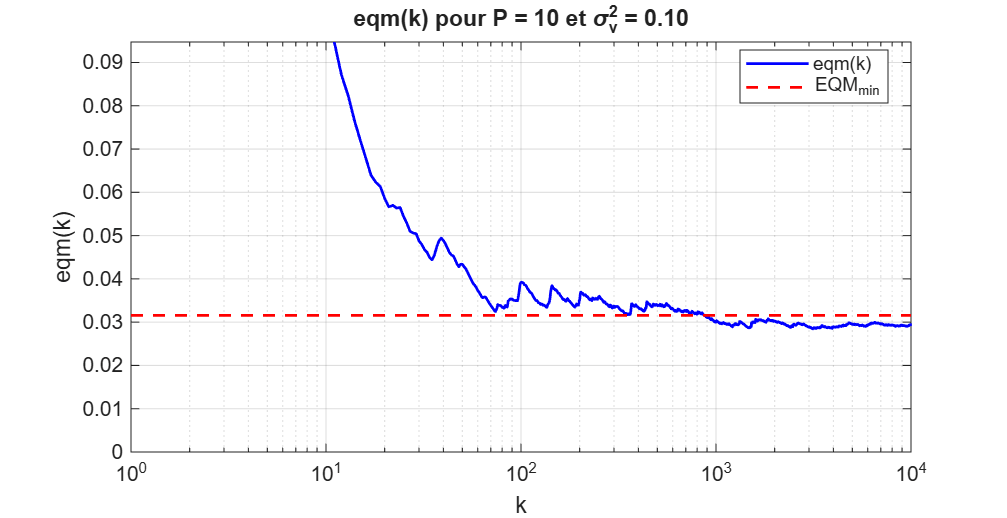
\includegraphics[width=\linewidth]{fig29}
    \caption{$\sigma_v^2=0.1$}
  \end{subfigure}\hfill
  \begin{subfigure}{0.49\linewidth}
    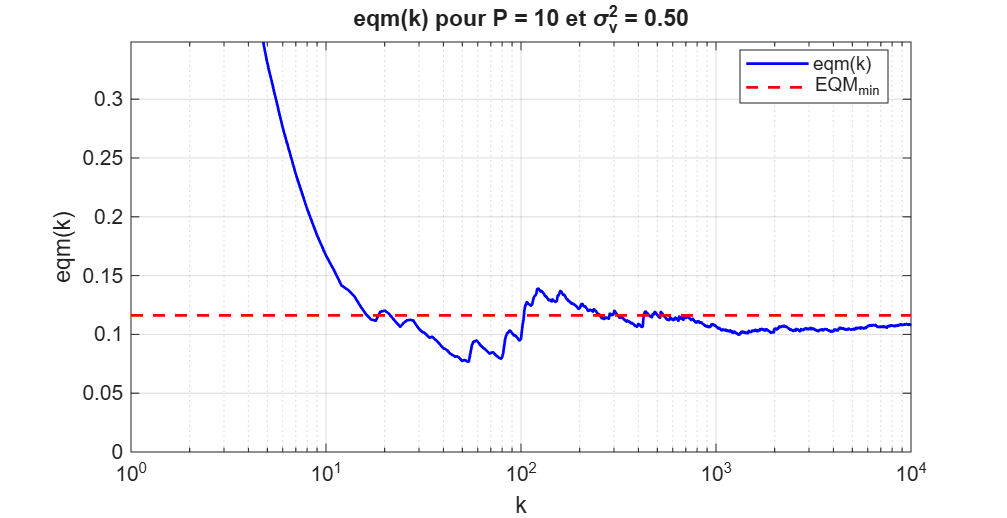
\includegraphics[width=\linewidth]{fig30}
    \caption{$\sigma_v^2=0.5$}
  \end{subfigure}

  \medskip
  \begin{subfigure}{0.49\linewidth}
    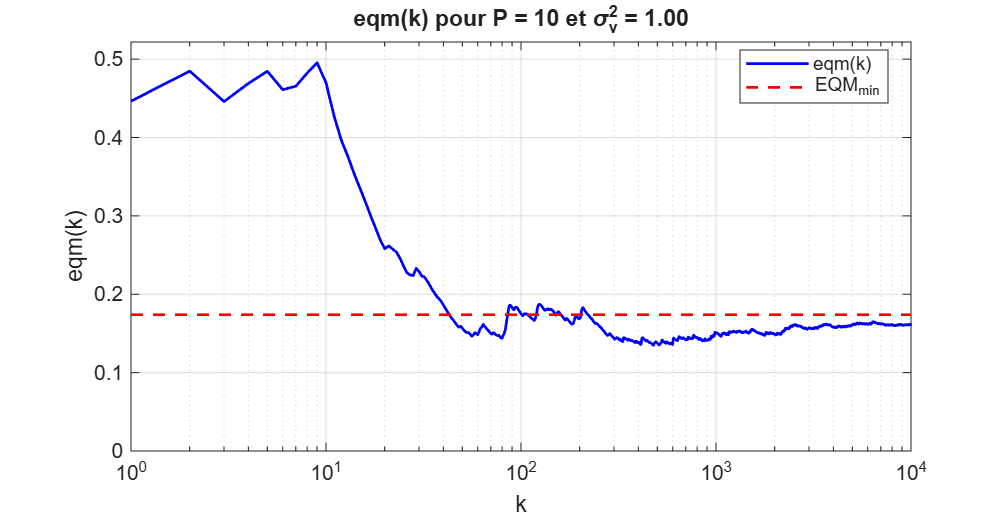
\includegraphics[width=\linewidth]{fig31}
    \caption{$\sigma_v^2=1$}
  \end{subfigure}
  \caption{$eqm(k)$ et $\mathrm{EQM}_{\min}$ pour $P=10$ et les différentes valeurs de $\sigma_v^2$ ($N=10^4$).}
\end{figure}

\begin{figure}[H]
  \centering
  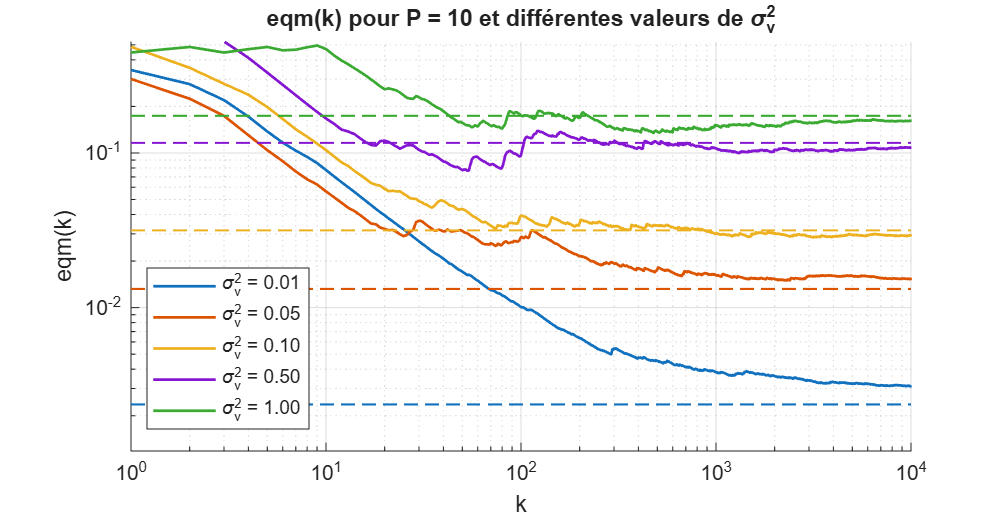
\includegraphics[width=0.8\linewidth]{fig32}
  \caption{Comparaison de $eqm(k)$ pour $P=10$ (pointillés : $\mathrm{EQM}_{\min}$ correspondants), $N=10^4$.}
  \label{fig:comp1e4}
\end{figure}

\begin{figure}[H]
  \centering
  \begin{subfigure}{0.49\linewidth}
    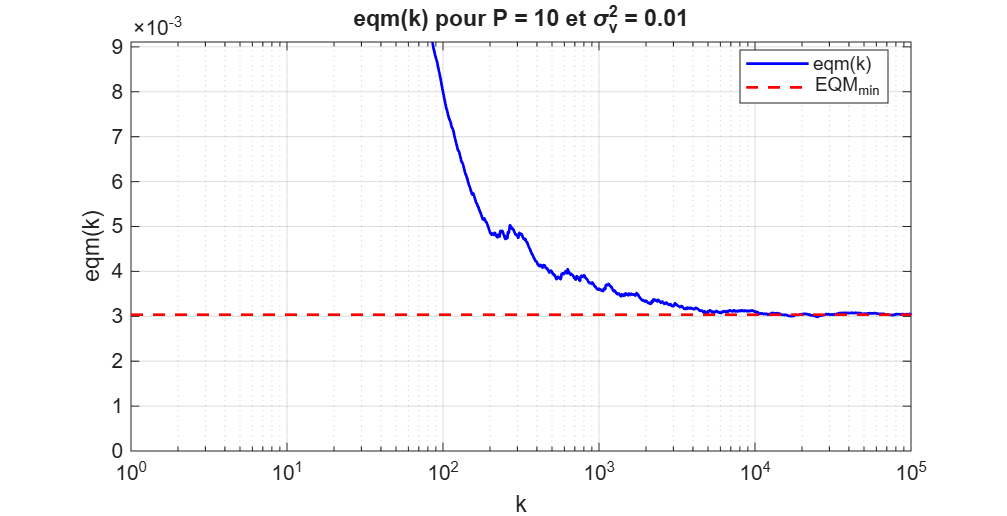
\includegraphics[width=\linewidth]{fig33}
    \caption{$\sigma_v^2=0.01$}
    \label{fig:verif1}
  \end{subfigure}\hfill
  \begin{subfigure}{0.49\linewidth}
    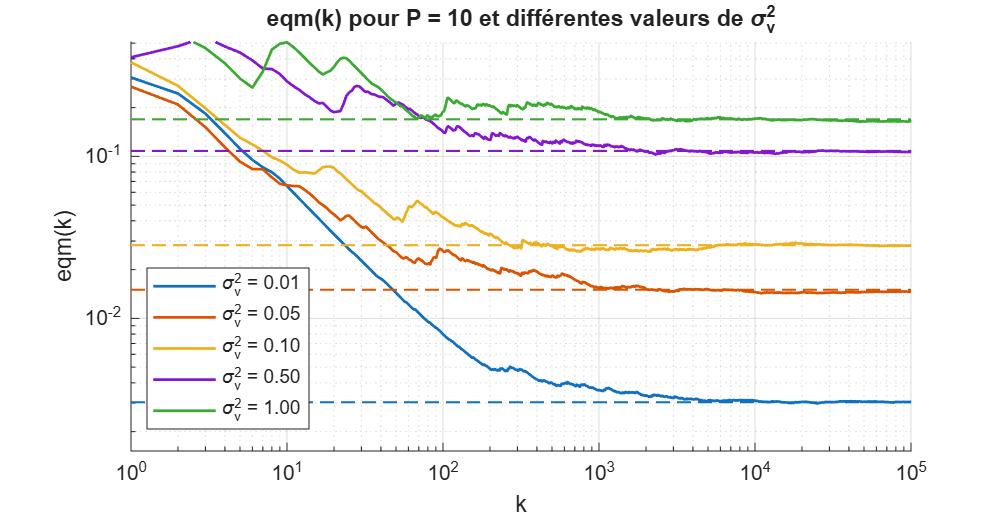
\includegraphics[width=\linewidth]{fig34}
    \caption{Toutes les valeurs de $\sigma_v^2$}
    \label{fig:verif2}
  \end{subfigure}
  \caption{Vérification avec $N=10^5$ échantillons ($P=10$).}
\end{figure}

\begin{table}[H]
  \centering
  \begin{tabular}{cccc}
    \toprule
    $\sigma_v^2$ & $\mathrm{EQM}_{\min}$ (formule, $N=10^4$) & $eqm(N)$ mesurée ($N=10^4$) & $\mathrm{EQM}_{\min}$ théorique \\
    \midrule
    $0.01$ & $0.0024$ & $0.0031$ & $0.0030$ \\
    $0.05$ & $0.013$  & $0.015$  & $0.015$ \\
    $0.1$  & $0.032$  & $0.029$  & $0.028$ \\
    $0.5$  & $0.116$  & $0.108$  & $0.107$ \\
    $1$    & $0.173$  & $0.161$  & $0.168$ \\
    \bottomrule
  \end{tabular}
  \caption{Erreurs obtenues pour $P=10$. La colonne théorique utilise les corrélations exactes $r_d(k)=\tfrac12\cos(kw_0)$ et $r_x(k)=r_d(k)+\sigma_v^2\delta(k)$.}
\end{table}

\begin{interpretation}
\begin{itemize}
  \item \textbf{Effet du bruit.} $\mathrm{EQM}_{\min}$ augmente avec $\sigma_v^2$ : avec $P=10$ coefficients, le résidu de bruit croît avec la puissance du bruit. Elle reste toujours inférieure à $\sigma_v^2$ (erreur sans filtrage) : le filtre réduit le bruit dans tous les cas.
  \item \textbf{Écart entre $eqm(N)$ et $\mathrm{EQM}_{\min}$.} Les courbes se stabilisent, mais pas exactement sur la droite (écart de signe variable). C'est une \emph{erreur d'estimation} de $\mathrm{EQM}_{\min}$ : la formule suppose $r_{dx}(k)=r_d(k)$, alors que l'intercorrélation estimée entre $d$ et $v$ n'est pas nulle sur $10^4$ échantillons. L'écart est négligeable à fort bruit mais important pour $\sigma_v^2=0.01$ ($0.0024$ contre $0.0031$).
  \item \textbf{Vérification ($N=10^5$).} Pour $\sigma_v^2=0.01$, $\mathrm{EQM}_{\min}$ passe à $0.0030$, égale à la valeur théorique, et $eqm(k)$ converge vers elle ; toutes les courbes rejoignent alors leur droite (figure~\ref{fig:verif2}). L'erreur d'estimation diminue donc quand $N$ augmente.
  \item \textbf{Vitesse de convergence.} Elle est plus lente à faible bruit : l'erreur initiale (transitoire), divisée par $k$, doit devenir négligeable devant une $\mathrm{EQM}_{\min}$ très petite ($k\approx 10^3$--$10^4$ pour $\sigma_v^2=0.01$, contre $10^2$--$10^3$ pour les autres).
\end{itemize}
\end{interpretation}

\subsection{Question (e) : \texorpdfstring{$\mathrm{EQM}_{\min}$}{EQMmin} en fonction de l'ordre P}

\begin{enonce}
\textbf{Énoncé :} On fixe $\sigma_v^2=0.1$. Tracer $\mathrm{EQM}_{\min}$ en fonction de $P$, pour $P$ variant de $5$ à $50$ avec un pas de $5$. Interpréter.
\end{enonce}

\textbf{Démarche.} Une seule réalisation de $x(n)$ est utilisée pour tous les ordres, afin que seul $P$ change. Pour chaque $P$, on calcule $\mathrm{EQM}_{\min}$ (formule) et, pour contrôle, l'erreur mesurée $eqm(N)$.

\textbf{Code.}
\begin{lstlisting}
clear; clc; close all;

% Parametres
N     = 1e4;
n     = (1:N)';
w0    = 0.05*pi;
phi   = pi/4;
sigv2 = 0.1;
Plist = 5:5:50;
nP    = length(Plist);

% Signal propre et signal bruite (meme realisation pour tous les P)
d = sin(n*w0 + phi);
x = d + sqrt(sigv2)*randn(N,1);

EQMmin = zeros(1, nP);
eqmN   = zeros(1, nP);

for m = 1:nP
    P = Plist(m);

    % Filtre de Wiener d'ordre P
    rx = xcorr(x, P-1, 'biased'); rx = rx(P:end);
    rd = xcorr(d, P-1, 'biased'); rd = rd(P:end);
    hopt = toeplitz(rx) \ rd;
    dhat = filter(hopt, 1, x);

    % EQM_min (formule)
    EQMmin(m) = rd(1) - hopt' * rd;

    % eqm(N) mesuree
    S = 0;
    for k = 1:N
        S = S + (d(k) - dhat(k))^2;
    end
    eqmN(m) = S / N;

    fprintf('P = %2d : EQM_min = %.4f | eqm(N) = %.4f\n', ...
            P, EQMmin(m), eqmN(m));
end

% EQM_min et eqm(N) en fonction de P
figure;
plot(Plist, EQMmin, 'b-o', 'LineWidth', 1.3, 'MarkerFaceColor', 'b'); hold on;
plot(Plist, eqmN, 'r--s', 'LineWidth', 1.3);
grid on; xticks(Plist);
xlabel('Ordre P'); ylabel('EQM');
legend('EQM_{min} (formule)', 'eqm(N) (mesuree)', 'Location', 'best');
\end{lstlisting}

\begin{figure}[H]
  \centering
  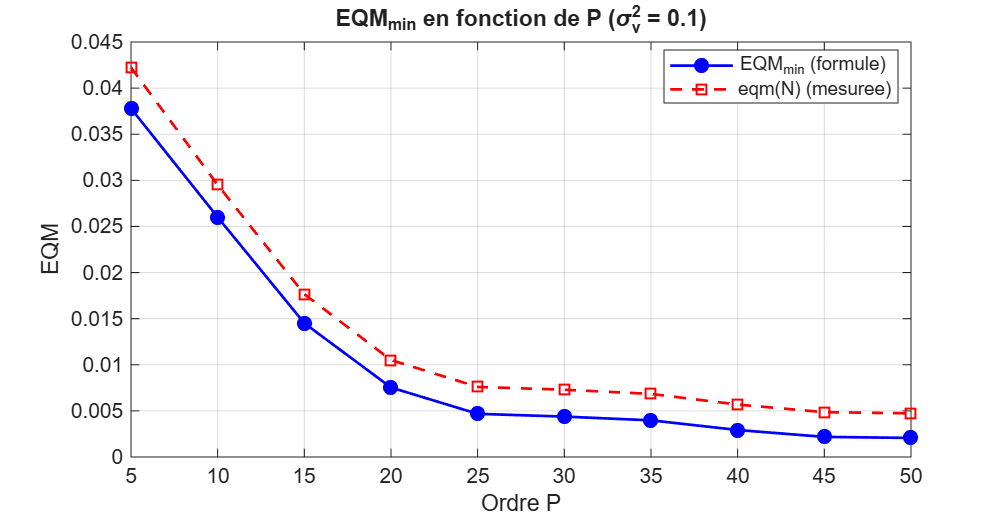
\includegraphics[width=0.8\linewidth]{fig35}
  \caption{$\mathrm{EQM}_{\min}$ (formule) et $eqm(N)$ (mesurée) en fonction de $P$ ($\sigma_v^2=0.1$).}
\end{figure}

\begin{interpretation}
\begin{itemize}
  \item \textbf{Tendance.} $\mathrm{EQM}_{\min}$ diminue avec $P$ : forte baisse de $P=5$ à $P=20$ ($0.0378\to 0.0075$, division par 5), puis palier ($0.0047$ à $P=25$, $0.0021$ à $P=50$).
  \item \textbf{Explication fréquentielle.} Le bruit blanc occupe toutes les fréquences, le signal est concentré en $w_0$. Un filtre plus long a une bande passante plus étroite autour de $w_0$ : il élimine plus de bruit sans toucher à la sinusoïde. Une fois la bande assez étroite, l'allonger n'apporte presque plus rien.
  \item \textbf{Mesure.} $eqm(N)$ suit la même tendance, avec un écart presque constant ($0.0045$ à $P=5$, $0.0026$ à $P=50$) : c'est l'erreur d'estimation vue en (d), de même signe ici car la réalisation du bruit est la même pour tous les $P$.
  \item \textbf{Conclusion.} Au-delà de $P\approx 25$, le gain en erreur est faible alors que le coût augmente (matrice $\mathbf{R}_x$ plus grande, transitoire plus long).
\end{itemize}
\end{interpretation}

\subsection{Question (f) : gain en RSB et choix de l'ordre P}

\begin{enonce}
\textbf{Énoncé :} Le gain en RSB après débruitage est défini par $\mathrm{gain}|_{\mathrm{dB}}=\mathrm{RSB}|_{\mathrm{ap}}-\mathrm{RSB}|_{\mathrm{av}}$. Afficher la courbe de $\mathrm{gain}|_{\mathrm{dB}}$ en faisant varier $P$ comme en (e). Interpréter. Quel est le meilleur choix de l'ordre $P$ ?
\end{enonce}

\textbf{Démarche.} Avant débruitage, l'erreur est $v(n)$ ; après, c'est $e(n)=d(n)-\hat d(n)$ :
\[
\mathrm{RSB}_{\mathrm{av}}=10\log_{10}\frac{P_d}{P_v},\qquad
\mathrm{RSB}_{\mathrm{ap}}=10\log_{10}\frac{P_d}{P_e},\qquad
\mathrm{gain}|_{\mathrm{dB}}=10\log_{10}\frac{P_v}{P_e}.
\]
Les puissances sont calculées par moyennes temporelles. On trace aussi le gain déduit de la formule, $10\log_{10}(P_v/\mathrm{EQM}_{\min})$.

\textbf{Code.}
\begin{lstlisting}
clear; clc; close all;

% Parametres
N     = 1e4;
n     = (1:N)';
w0    = 0.05*pi;
phi   = pi/4;
sigv2 = 0.1;
Plist = 5:5:50;
nP    = length(Plist);

% Signal propre et signal bruite (meme realisation pour tous les P)
d = sin(n*w0 + phi);
v = sqrt(sigv2)*randn(N,1);
x = d + v;

% Puissances du signal et du bruit
Sd = 0; Sv = 0;
for k = 1:N
    Sd = Sd + d(k)^2;
    Sv = Sv + v(k)^2;
end
Pd = Sd / N;
Pv = Sv / N;

% RSB avant debruitage
RSBav = 10*log10(Pd / Pv);

RSBap  = zeros(1, nP);
gain   = zeros(1, nP);
gainTh = zeros(1, nP);

for m = 1:nP
    P = Plist(m);

    % Filtre de Wiener d'ordre P
    rx = xcorr(x, P-1, 'biased'); rx = rx(P:end);
    rd = xcorr(d, P-1, 'biased'); rd = rd(P:end);
    hopt = toeplitz(rx) \ rd;
    dhat = filter(hopt, 1, x);
    EQMmin = rd(1) - hopt' * rd;

    % Puissance de l'erreur residuelle
    Se = 0;
    for k = 1:N
        Se = Se + (d(k) - dhat(k))^2;
    end
    Pe = Se / N;

    % RSB apres debruitage et gain
    RSBap(m)  = 10*log10(Pd / Pe);
    gain(m)   = RSBap(m) - RSBav;
    gainTh(m) = 10*log10(Pv / EQMmin);
end

% Gain en fonction de P
figure;
plot(Plist, gain, 'b-o', 'LineWidth', 1.3, 'MarkerFaceColor', 'b'); hold on;
plot(Plist, gainTh, 'r--s', 'LineWidth', 1.3);
grid on; xticks(Plist);
xlabel('Ordre P'); ylabel('gain (dB)');
legend('gain mesure', 'gain deduit de EQM_{min}', 'Location', 'best');
\end{lstlisting}

\begin{figure}[H]
  \centering
  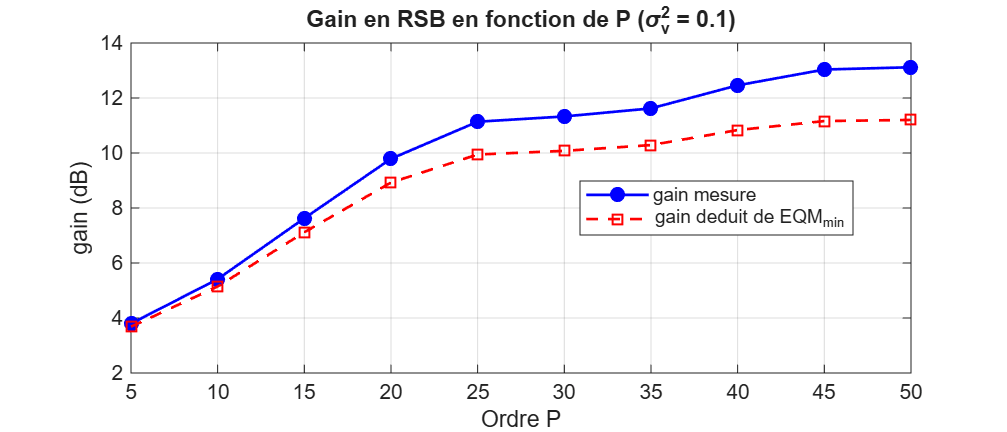
\includegraphics[width=0.8\linewidth]{fig36}
  \caption{Gain en RSB (mesuré et déduit de $\mathrm{EQM}_{\min}$) en fonction de $P$ ($\sigma_v^2=0.1$).}
\end{figure}

\begin{interpretation}
\begin{itemize}
  \item \textbf{RSB initial.} $P_d=0.5$, $P_v=0.098$, donc $\mathrm{RSB}_{\mathrm{av}}=7.08$~dB.
  \item \textbf{Évolution du gain.} $3.80$~dB ($P=5$), $5.4$~dB ($P=10$), $9.79$~dB ($P=20$), $11.14$~dB ($P=25$), puis seulement $13.12$~dB à $P=50$. Comme $\mathrm{gain}|_{\mathrm{dB}}=10\log_{10}(P_v/P_e)$, la courbe est le miroir de celle de (e) : forte hausse, puis palier.
  \item \textbf{Gain déduit de $\mathrm{EQM}_{\min}$.} Même tendance, mais en dessous du gain mesuré (écart de $0.1$~dB à $P=5$ à $1.9$~dB à $P=50$). L'écart est de sens inverse de celui de (e), car ce script utilise une autre réalisation du bruit : c'est bien une erreur d'estimation aléatoire, plus visible en dB quand l'erreur est petite (grands $P$).
\end{itemize}
\end{interpretation}

\begin{resultat}[Meilleur choix de l'ordre]
$P\approx 25$ : environ $11$~dB de gain, soit l'essentiel de l'amélioration possible. Au-delà, doubler l'ordre n'apporte que $\approx 2$~dB (du même ordre que l'incertitude d'estimation) pour un coût de calcul et un transitoire plus grands.
\end{resultat}

%==================== PARTIE 3 ====================
\section{Partie 3 : Débruitage d'un signal audio}

Le signal de référence $d(n)$ est un enregistrement d'ambiance de plage (vagues et chants d'oiseaux), lu dans \texttt{monson.wav} ($F_s=44100$~Hz). On garde un canal et $N=10^5$ échantillons ($\approx 2.27$~s), en sautant la première seconde (silence). Le bruitage est celui de la partie~2 : $x(n)=d(n)+v(n)$, $v(n)\sim\mathcal{N}(0,\sigma_v^2)$, avec \texttt{rng(0)} pour des résultats reproductibles.

\textbf{Normalisation.} Le signal brut est très faible ($P_d\approx 0.0016$) : avec $\sigma_v^2=0.1$, le bruit serait 60 fois plus puissant et le filtre rendrait une sortie quasi nulle ($\mathrm{EQM}_{\min}=0.0015\approx P_d$). On normalise donc : $d(n)\leftarrow d(n)/\max|d(n)|$, comme la sinusoïde de la partie~2.

\subsection{Question préliminaire : RSB de 0 dB}

\begin{enonce}
\textbf{Énoncé :} Quelle valeur de $\sigma_v^2$ permet d'avoir un RSB avant débruitage de 0~dB ?
\end{enonce}

\textbf{Démarche.}
\[
\mathrm{RSB}_{\mathrm{av}}=10\log_{10}\frac{P_d}{\sigma_v^2}=0~\text{dB}
\iff \sigma_v^2=P_d=r_d(0)=\frac{1}{N}\sum_{n=1}^{N}d^2(n).
\]

\textbf{Code.}
\begin{lstlisting}
clear; clc; close all;
rng(0);                              % bruit reproductible

[y, Fs] = audioread('monson.wav');   % lecture du son
y = y(:,1);                          % un seul canal

N     = 1e5;
debut = round(1*Fs);                 % on saute la 1re seconde
d = y(debut+1 : debut+N);            % signal de reference
d = d / max(abs(d));                 % normalisation dans [-1, 1]

% Puissance du signal r_d(0)
Sd = 0;
for k = 1:N
    Sd = Sd + d(k)^2;
end
Pd = Sd / N;
fprintf('Pd = %.4f -> sigma_v^2 pour RSB = 0 dB : %.4f\n', Pd, Pd);
\end{lstlisting}

\begin{resultat}
$P_d=0.0411$, donc $\boldsymbol{\sigma_v^2=0.0411}$ donne un RSB de 0~dB.
\end{resultat}

\begin{interpretation}
La puissance du signal audio normalisé est 12 fois plus faible que celle de la sinusoïde ($0.5$) : il reste la plupart du temps proche de zéro, avec quelques pics. Avec $\sigma_v^2=0.1$, le RSB de départ est donc négatif.
\end{interpretation}

\subsection{Question (a) : \texorpdfstring{$\mathrm{EQM}_{\min}$ pour $P=10$ et $\sigma_v^2=0.1$}{EQMmin pour P = 10}}

\begin{enonce}
\textbf{Énoncé :} Afin d'évaluer la performance du débruitage, calculer $\mathrm{EQM}_{\min}=r_d(0)-\mathbf{w}_{opt}^T\mathbf{r}_{dx}$ pour $P=10$ et $\sigma_v^2=0.1$.
\end{enonce}

\textbf{Démarche.} Bruitage, calcul de $\mathbf{w}_{opt}$ et de $\hat d(n)$ comme en partie~2, puis de $\mathrm{EQM}_{\min}$. Pour juger la performance, on la compare à l'erreur sans filtrage ($\sigma_v^2$) et à l'erreur d'une sortie nulle ($P_d$), et on calcule le gain $\mathrm{gain}|_{\mathrm{dB}}=10\log_{10}(P_d/\mathrm{EQM}_{\min})-10\log_{10}(P_d/\sigma_v^2)$.

\textbf{Code.} (à la suite du code précédent)
\begin{lstlisting}
P = 10;  sigv2 = 0.1;

x = d + sqrt(sigv2)*randn(N,1);      % signal bruite

% Filtre de Wiener : r_dx(k) = r_d(k)
rx = xcorr(x, P-1, 'biased'); rx = rx(P:end);
rd = xcorr(d, P-1, 'biased'); rd = rd(P:end);
hopt = toeplitz(rx) \ rd;
dhat = filter(hopt, 1, x);           % signal debruite

% EQM minimale (rd(1) correspond a r_d(0))
EQMmin = rd(1) - hopt'*rd;
fprintf('EQM_min = %.4f (bruit avant filtrage : %.2f)\n', EQMmin, sigv2);

% RSB avant / apres et gain
RSB_av = 10*log10(rd(1)/sigv2);
RSB_ap = 10*log10(rd(1)/EQMmin);
fprintf('RSB avant = %.2f dB | RSB apres = %.2f dB | gain = %.2f dB\n', ...
        RSB_av, RSB_ap, RSB_ap - RSB_av);

% Affichage d'une fenetre
idx = 1001:1300;
figure;
plot(idx, x(idx), 'Color', [0.7 0.7 0.7]); hold on;
plot(idx, d(idx), 'b', 'LineWidth', 1.2);
plot(idx, dhat(idx), 'r', 'LineWidth', 1.2);
grid on; xlabel('n'); ylabel('Amplitude');
legend('x(n) : signal bruite', 'd(n) : signal propre', ...
       'dhat(n) : signal debruite');
saveas(gcf, 'figs_partie3/p3_qa_signaux.png');

% Ecoute
sound(d, Fs);    pause(N/Fs + 0.5);
sound(x, Fs);    pause(N/Fs + 0.5);
sound(dhat, Fs);
\end{lstlisting}

\begin{figure}[H]
  \centering
  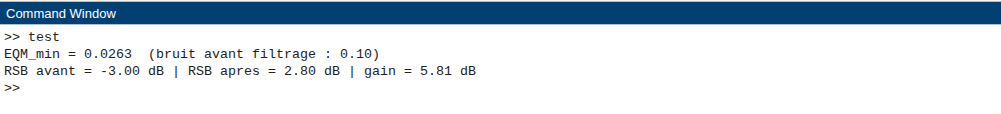
\includegraphics[width=0.75\linewidth]{p3_qa_resultats}
  \caption{Valeurs de $P_d$, $\mathrm{EQM}_{\min}$, des RSB et du gain ($P=10$, $\sigma_v^2=0.1$).}
\end{figure}

\begin{figure}[H]
  \centering
  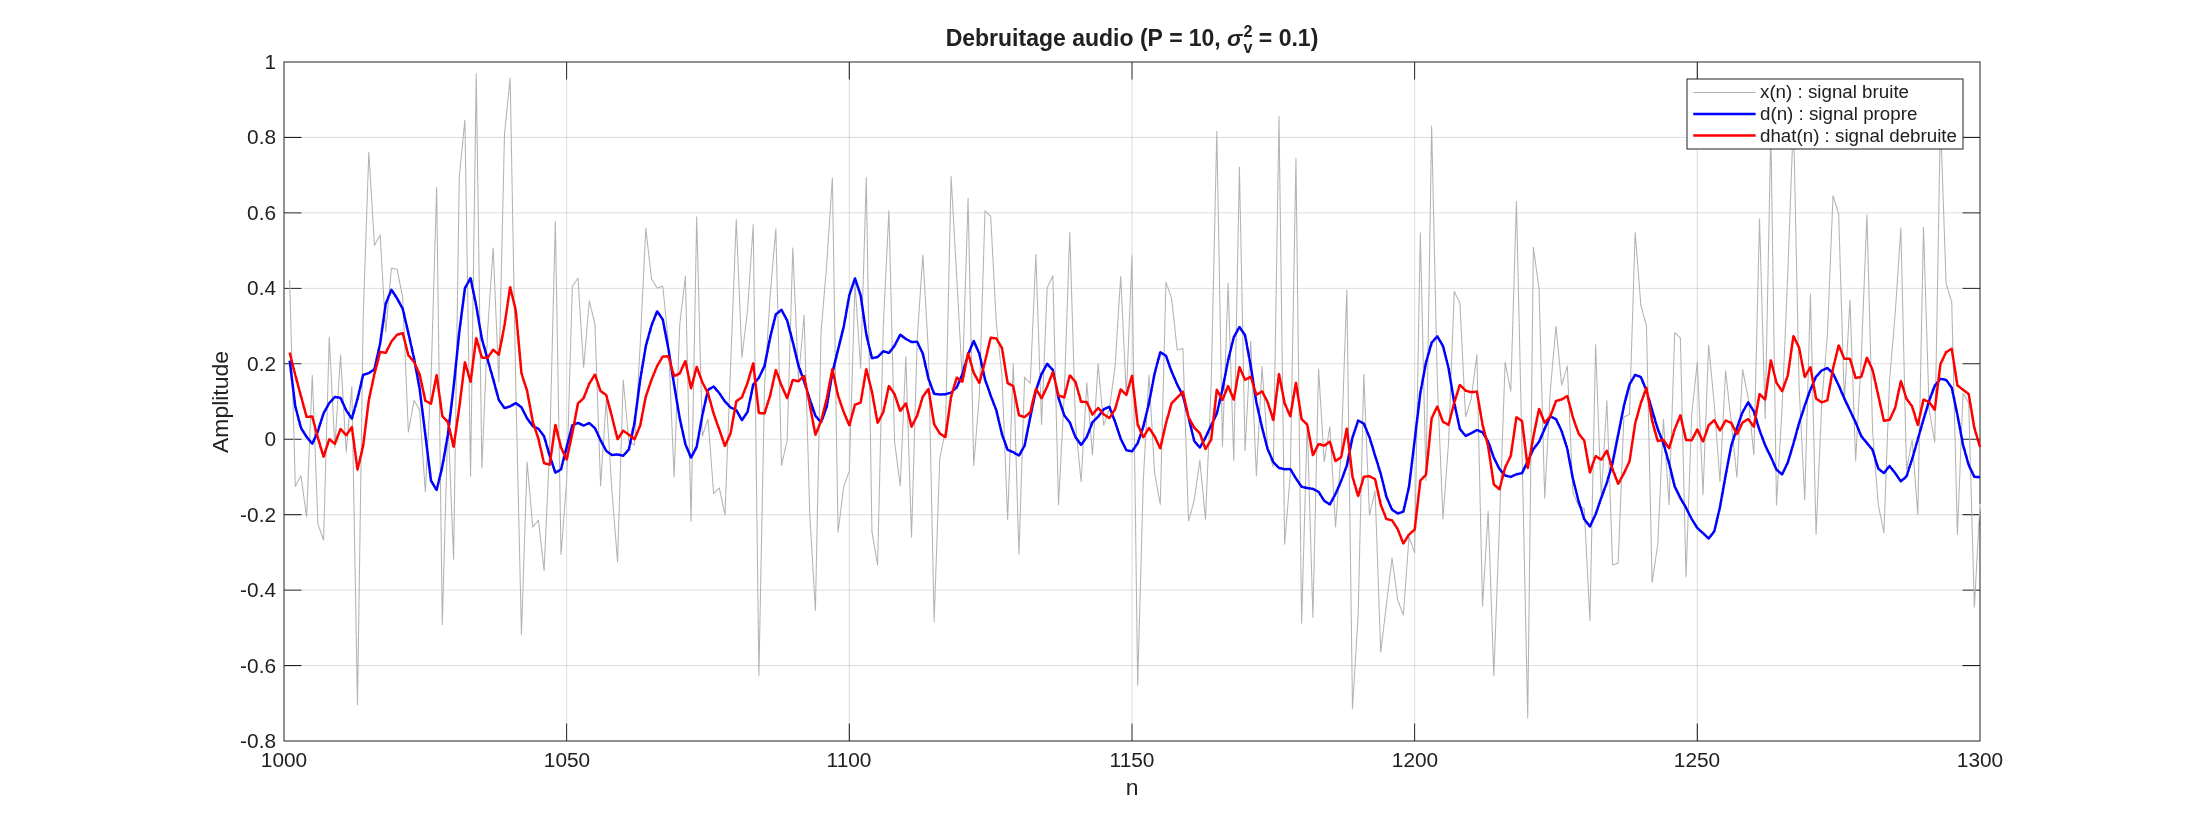
\includegraphics[width=\linewidth]{p3_qa_signaux}
  \caption{Signal bruité $x(n)$, signal propre $d(n)$ et signal débruité $\hat d(n)$ ($P=10$, $\sigma_v^2=0.1$).}
\end{figure}

\begin{resultat}
$\mathrm{EQM}_{\min}=0.0155$ ; $\mathrm{RSB}_{\mathrm{av}}\approx-3.9$~dB, $\mathrm{RSB}_{\mathrm{ap}}\approx 4.2$~dB, soit un gain d'environ $8.1$~dB.
\end{resultat}

\begin{interpretation}
\begin{itemize}
  \item \textbf{Performance.} L'erreur passe de $0.1$ (sans filtrage) à $0.0155$. Elle est aussi bien inférieure à celle d'une sortie nulle ($P_d=0.0411$) : le filtre récupère réellement une partie du signal.
  \item \textbf{Allure.} $\hat d(n)$ suit l'allure de $d(n)$ et est beaucoup plus lisse que $x(n)$, mais les pics sont atténués et légèrement retardés : le filtre est une moyenne pondérée des $P$ derniers échantillons.
  \item \textbf{Comparaison avec la partie~2.} Le gain est supérieur à celui de la sinusoïde pour $P=10$ ($5.4$~dB), mais le RSB de départ est très différent ($-3.9$~dB contre $7$~dB) : le gain augmente mécaniquement quand le bruit domine (voir (c), (d) et (f)).
  \item \textbf{Écoute.} Les vagues (basses fréquences) sont conservées, les chants d'oiseaux (aigus) sont atténués avec le bruit : le filtre se comporte en passe-bas.
\end{itemize}
\end{interpretation}

\subsection{Question (b) : reprise des questions (e) et (f) de la partie 2}

\begin{enonce}
\textbf{Énoncé :} Reprendre les questions (e) et (f) de la partie~2 : pour $\sigma_v^2=0.1$, tracer $\mathrm{EQM}_{\min}$ puis le gain en RSB en fonction de $P$ (de 5 à 50, pas de 5). Choisir le meilleur ordre $P$.
\end{enonce}

\textbf{Démarche.} Un seul signal bruité pour tous les $P$. Les corrélations sont estimées une fois jusqu'au retard $49$ ; pour chaque $P$ on garde les $P$ premiers retards et on calcule $\mathrm{EQM}_{\min}$ et $\mathrm{gain}|_{\mathrm{dB}}=10\log_{10}(\sigma_v^2/\mathrm{EQM}_{\min})$.

\textbf{Code.}
\begin{lstlisting}
clear; clc; close all;
rng(0);

% Signal (comme en (a))
[y, Fs] = audioread('monson.wav');
y = y(:,1);
N = 1e5;  debut = round(1*Fs);
d = y(debut+1 : debut+N);
d = d / max(abs(d));

sigv2 = 0.1;
x = d + sqrt(sigv2)*randn(N,1);      % meme bruit pour tous les P

Plist  = 5:5:50;
EQMmin = zeros(size(Plist));
gain   = zeros(size(Plist));

% Correlations calculees une seule fois jusqu'au retard max
Pmax = max(Plist);
rxF = xcorr(x, Pmax-1, 'biased'); rxF = rxF(Pmax:end);
rdF = xcorr(d, Pmax-1, 'biased'); rdF = rdF(Pmax:end);

RSB_av = 10*log10(rdF(1)/sigv2);

for m = 1:length(Plist)
    P  = Plist(m);
    rx = rxF(1:P);  rd = rdF(1:P);   % P premiers retards
    hopt = toeplitz(rx) \ rd;
    EQMmin(m) = rd(1) - hopt'*rd;
    gain(m)   = 10*log10(rd(1)/EQMmin(m)) - RSB_av;
    fprintf('P = %2d : EQM_min = %.5f | gain = %.2f dB\n', ...
            P, EQMmin(m), gain(m));
end

% EQM_min en fonction de P
figure;
plot(Plist, EQMmin, 'bo-', 'LineWidth', 1.3); grid on;
xlabel('P'); ylabel('EQM_{min}');
saveas(gcf, 'figs_partie3/p3_qb_eqm.png');

% Gain en fonction de P
figure;
plot(Plist, gain, 'ro-', 'LineWidth', 1.3); grid on;
xlabel('P'); ylabel('gain (dB)');
saveas(gcf, 'figs_partie3/p3_qb_gain.png');
\end{lstlisting}

\begin{figure}[H]
  \centering
  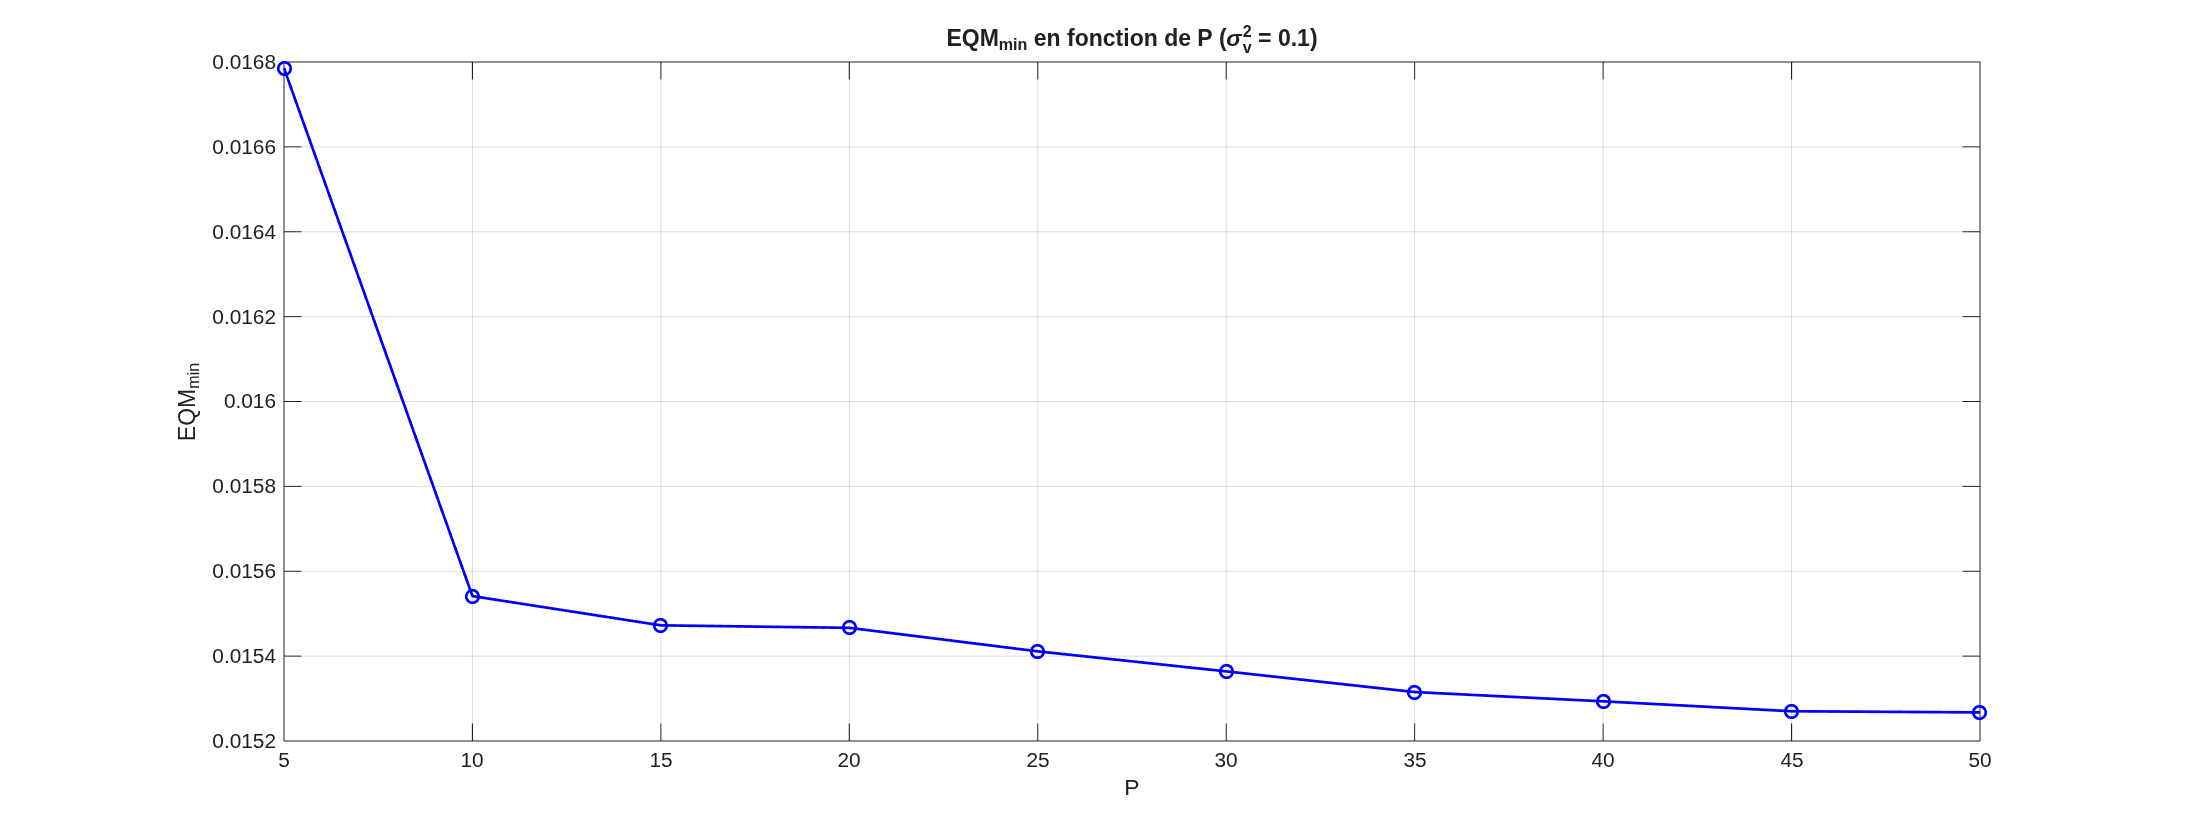
\includegraphics[width=\linewidth]{p3_qb_eqm}
  \caption{$\mathrm{EQM}_{\min}$ en fonction de $P$ ($\sigma_v^2=0.1$, signal audio).}
\end{figure}

\begin{figure}[H]
  \centering
  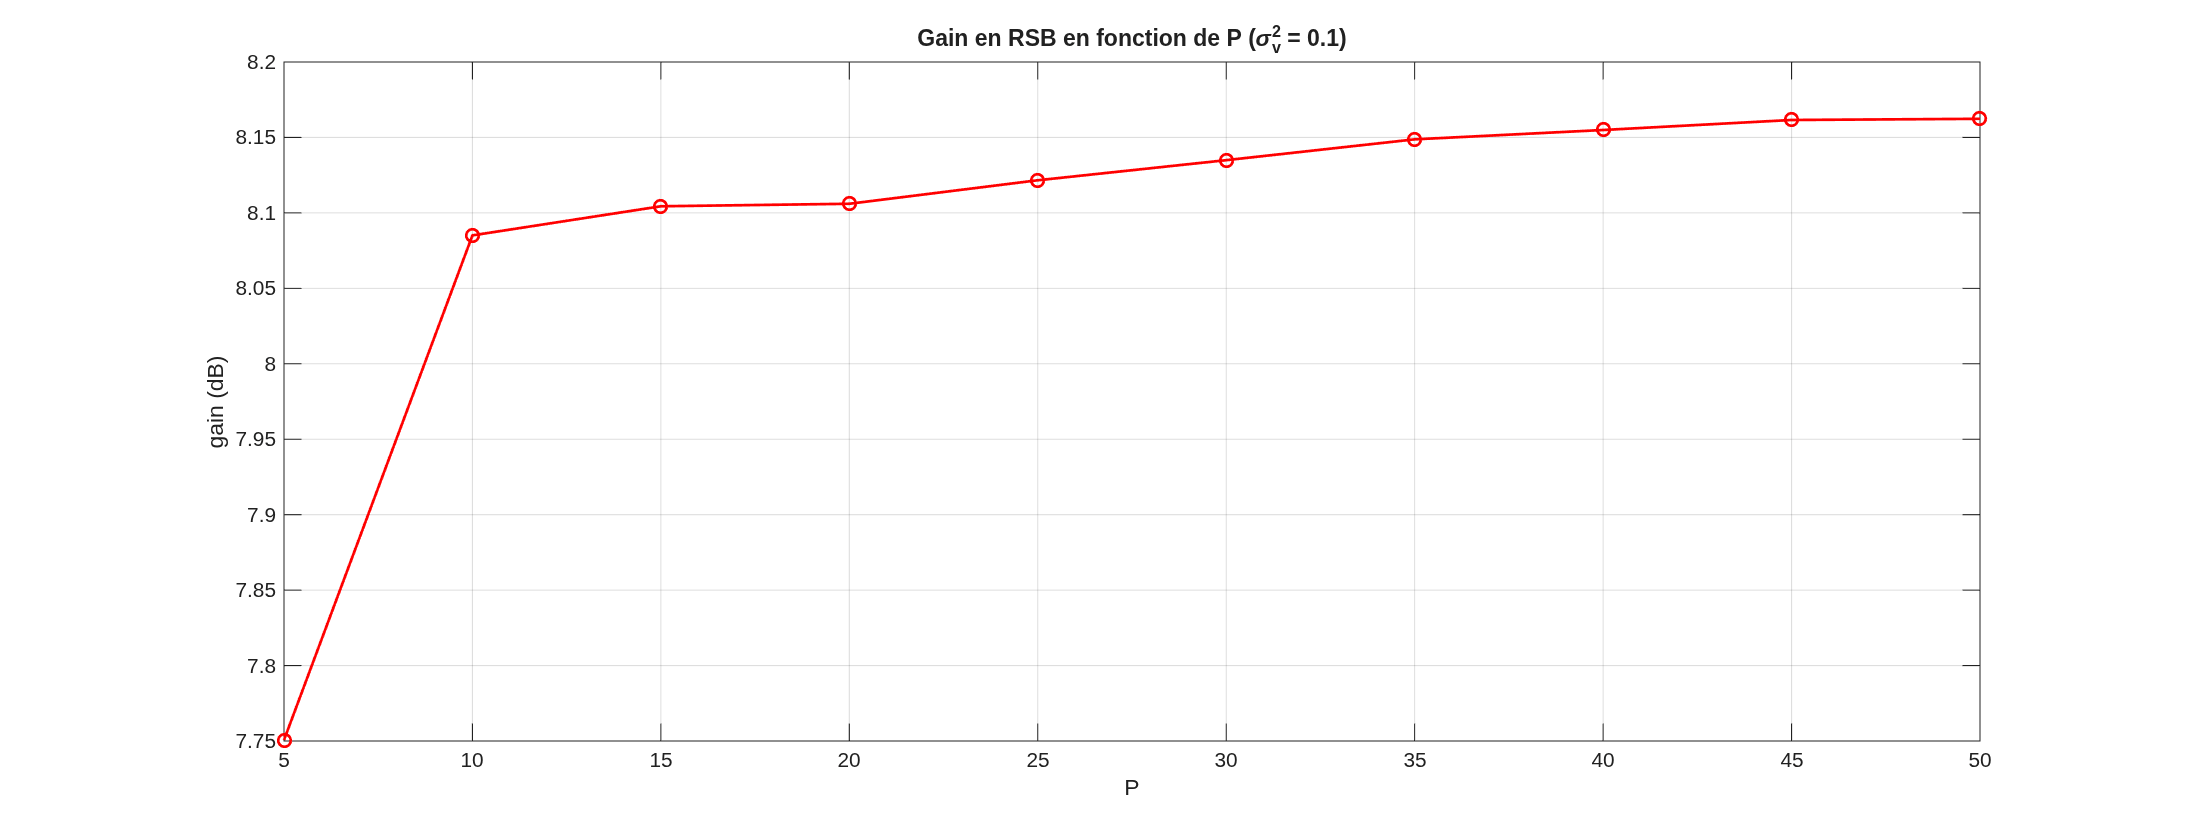
\includegraphics[width=\linewidth]{p3_qb_gain}
  \caption{Gain en RSB en fonction de $P$ ($\sigma_v^2=0.1$, signal audio).}
\end{figure}

\begin{interpretation}
\begin{itemize}
  \item \textbf{Évolution.} $\mathrm{EQM}_{\min}$ passe de $0.0168$ ($P=5$) à $0.0155$ ($P=10$), puis à $0.0153$ ($P=50$). Le gain passe de $7.75$ à $8.09$~dB, puis ne gagne que $0.08$~dB jusqu'à $P=50$. Attention à l'échelle zoomée : le gain ne varie que de $0.4$~dB sur toute la plage. Pour $P=10$, on retrouve le gain de (a) (même bruit grâce à \texttt{rng(0)}).
  \item \textbf{Explication.} La corrélation du signal audio décroît vite : les échantillons éloignés n'apportent presque plus d'information. À $F_s=44100$~Hz, 10 échantillons ($\approx 0.23$~ms) suffisent à exploiter l'essentiel de cette corrélation. Pour la sinusoïde, dont la corrélation ne décroît pas, le palier n'était atteint que vers $P=25$.
\end{itemize}
\end{interpretation}

\begin{resultat}[Meilleur choix de l'ordre]
$P=10$ : c'est le coude des courbes, le plus petit ordre donnant presque le gain maximal. Un ordre plus grand augmente le coût de calcul pour un gain négligeable.
\end{resultat}

\subsection{Question (c) : débruitage par trames de 3 ms}

\begin{enonce}
\textbf{Énoncé :} Réaliser le débruitage par trames de 3~ms : sur chaque trame $i$, filtre de Wiener $\mathbf{w}^i_{opt}=(\mathbf{R}^i_x)^{-1}\mathbf{r}^i_{d}$, où $\mathbf{R}^i_x$ est la matrice d'autocorrélation de la trame $i$ du signal bruité et $\mathbf{r}^i_{d}$ le vecteur d'autocorrélation de la trame $i$ du signal de référence, pour $P=10$ et $\sigma_v^2=0.5$. Donner le code (fonction \texttt{debruitage\_sig}), afficher $\mathrm{gain}|_{\mathrm{dB}}$ en fonction du numéro de trame $i$ et le comparer au gain obtenu sur tout le signal. Donner la ou les lignes de code permettant de reconstruire le signal à partir des trames débruitées.
\end{enonce}

\textbf{Démarche.}
\begin{enumerate}
  \item \textbf{Découpage.} $L=\mathrm{round}(3\cdot10^{-3}F_s)=132$ échantillons par trame, soit $K=\lfloor N/L\rfloor=757$ trames (les $76$ derniers échantillons sont ignorés).
  \item \textbf{Fonction \texttt{debruitage\_sig(d, P, sigv2)}} : bruite la trame, estime $r_x(k)$ et $r_d(k)$ sur la trame seule, calcule $\mathbf{w}_{opt}$, filtre, et renvoie $x$, $\hat d$, $\mathrm{gain}|_{\mathrm{dB}}=10\log_{10}(P_v/P_e)$ et $\mathrm{EQM}_{\min}$.
  \item \textbf{Débruitage par trames} : appel sur chaque trame et replacement des trames débruitées à leur position.
  \item \textbf{Référence} : même fonction appliquée à tout le signal (un seul filtre).
\end{enumerate}

\textbf{Code.} Fonction de débruitage (\texttt{debruitage\_sig.m}) :
\begin{lstlisting}
function [x, dhat, gain_dB, EQMmin] = debruitage_sig(d, P, sigv2)
% Debruitage d'un signal d par filtre de Wiener d'ordre P
% Entrees : d (signal propre), P (ordre), sigv2 (variance du bruit)
% Sorties : x (signal bruite), dhat (signal debruite), gain en dB, EQM_min
d = d(:);
N = length(d);
v = sqrt(sigv2)*randn(N,1);          % bruit blanc gaussien
x = d + v;                           % signal bruite

rx = xcorr(x, P-1, 'biased'); rx = rx(P:end);
rd = xcorr(d, P-1, 'biased'); rd = rd(P:end);
hopt = toeplitz(rx) \ rd;            % filtre de Wiener
dhat = filter(hopt, 1, x);           % signal debruite
EQMmin = rd(1) - hopt'*rd;           % EQM minimale (formule)

% Gain mesure : erreur avant (bruit) / erreur apres (residu)
Pd     = rd(1);
RSB_av = 10*log10(Pd / mean(v.^2));
RSB_ap = 10*log10(Pd / mean((d - dhat).^2));
gain_dB = RSB_ap - RSB_av;
end
\end{lstlisting}

Script principal (\texttt{p3\_qc.m}) :
\begin{lstlisting}
clear; clc; close all;
rng(0);

% Signal
[y, Fs] = audioread('monson.wav');
y = y(:,1);
N = 1e5;  debut = round(1*Fs);
d = y(debut+1 : debut+N);
d = d / max(abs(d));
P = 10;  sigv2 = 0.5;

% Decoupage en trames de 3 ms
L = round(3e-3 * Fs);                % 132 echantillons par trame
K = floor(N / L);                    % nombre de trames
fprintf('L = %d echantillons/trame | K = %d trames\n', L, K);

gains    = zeros(K,1);
EQMs     = zeros(K,1);
x_rec    = zeros(K*L,1);
dhat_rec = zeros(K*L,1);

% Debruitage trame par trame
for i = 1:K
    idx = (i-1)*L+1 : i*L;           % indices de la trame i
    [xi, dhi, gains(i), EQMs(i)] = debruitage_sig(d(idx), P, sigv2);
    x_rec(idx)    = xi;              % reconstruction du signal bruite
    dhat_rec(idx) = dhi;             % reconstruction du signal debruite
end

% Debruitage sur tout le signal (reference)
[x_g, dhat_g, gain_g, EQM_g] = debruitage_sig(d, P, sigv2);
fprintf('Gain global (tout le signal)  = %.2f dB\n', gain_g);
fprintf('Gain moyen par trame          = %.2f dB\n', mean(gains));

% Gain par trame
figure;
plot(1:K, gains, 'b.-'); hold on;
yline(gain_g, 'r--', 'LineWidth', 1.5);
yline(mean(gains), 'k:', 'LineWidth', 1.5);
grid on; xlabel('numero de trame i'); ylabel('gain (dB)');
legend('gain par trame', 'gain global', 'gain moyen par trame');
saveas(gcf, 'figs_partie3/p3_qc_gain_trames.png');

% Ecoute : debruitage global puis par trames
sound(dhat_g, Fs);    pause(N/Fs + 0.5);
sound(dhat_rec, Fs);
\end{lstlisting}

\begin{resultat}[Reconstruction du signal]
Chaque trame débruitée est replacée à sa position dans la boucle :
\begin{lstlisting}[numbers=none]
idx = (i-1)*L+1 : i*L;
dhat_rec(idx) = dhi;
\end{lstlisting}
\end{resultat}

\begin{figure}[H]
  \centering
  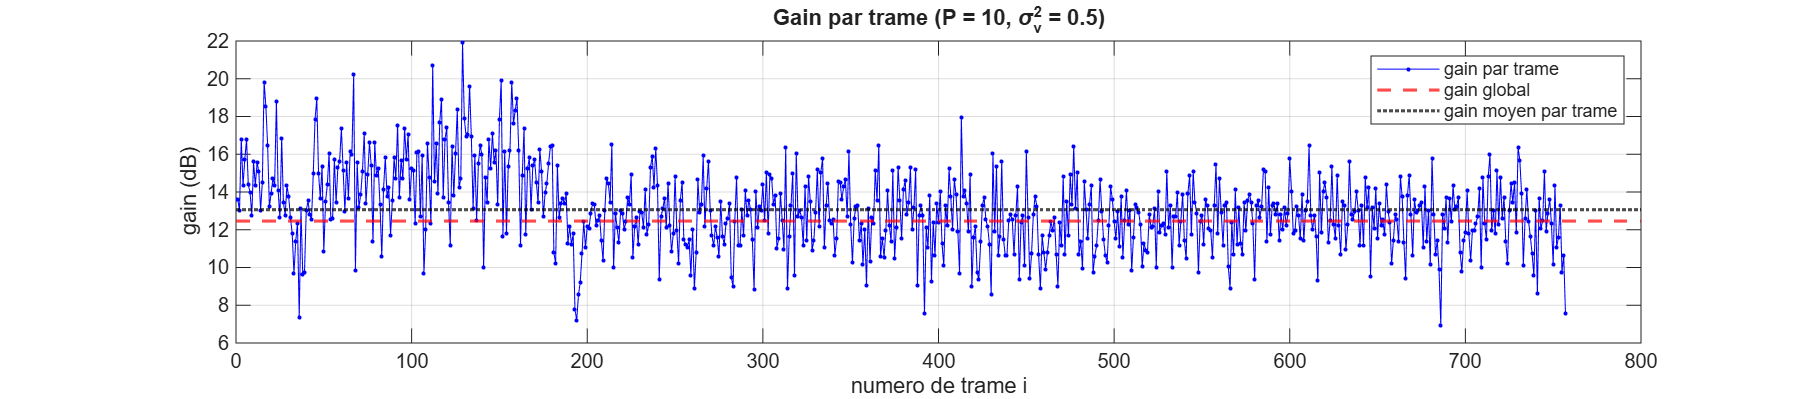
\includegraphics[width=\linewidth]{p3_qc_gain_trames}
  \caption{Gain en RSB de chaque trame de 3~ms, comparé au gain global et au gain moyen par trame ($P=10$, $\sigma_v^2=0.5$).}
\end{figure}

\begin{resultat}
$K=757$ trames de $L=132$ échantillons. Gain global : $12.46$~dB ; gain moyen par trame : $13.06$~dB (+0.6~dB).
\end{resultat}

\begin{interpretation}
\begin{itemize}
  \item \textbf{Comparaison.} Le gain moyen par trame dépasse le gain global : le signal audio n'est pas stationnaire (vagues, chants d'oiseaux), un filtre par trame s'adapte aux statistiques locales, alors qu'un filtre unique est un compromis moyen. Sur 3~ms, le signal est à peu près stationnaire, ce qui justifie le filtre de Wiener.
  \item \textbf{Dispersion.} La plupart des trames sont entre $10$ et $16$~dB, avec des chutes vers $7$~dB (trames $\approx 40$, $200$, $690$) et des pics à $20$--$22$~dB dans les $150$ premières trames. Causes : contenu variable d'une trame à l'autre (le gain dépend de la puissance de la trame, voir (d)), corrélations estimées sur seulement $132$ échantillons, et transitoire de $P-1=9$ échantillons ($7\,\%$ de la trame) car le filtre redémarre à zéro à chaque trame.
  \item \textbf{Nuances.} La moyenne de gains en dB n'est pas le gain du signal reconstruit (en (e), l'écart réel n'est que de $\approx 0.2$~dB) ; le traitement par trames coûte $757$ résolutions de systèmes au lieu d'une.
  \item \textbf{Gain global plus élevé qu'en (a)} ($12.46$ contre $8.1$~dB) : non pas parce que le signal est mieux reconstruit, mais parce que l'erreur reste bornée par $\approx P_d$ alors que $P_v$ augmente ; le gain croît donc mécaniquement avec le bruit.
\end{itemize}
\end{interpretation}

\subsection{Question (d) : étude statistique du gain et de \texorpdfstring{$\mathrm{EQM}_{\min}$}{EQMmin} par trame}

\begin{enonce}
\textbf{Énoncé :} Faire de même pour $\mathrm{EQM}_{\min}$ en comparant les résultats des différentes trames. Donner une description statistique des valeurs de $\mathrm{gain}|_{\mathrm{dB}}$ et $\mathrm{EQM}_{\min}$ et interpréter. Quelle fonction MATLAB peut-on utiliser pour décrire la distribution des valeurs ?
\end{enonce}

\textbf{Démarche.} Même découpage et même bruit qu'en (c). Pour chaque trame : $\mathrm{gain}|_{\mathrm{dB}}$, $\mathrm{EQM}^i_{\min}$ et la puissance $P^i_d$. Statistiques : moyenne, écart-type, médiane, min, max, quartiles $Q_1$ et $Q_3$ ; distributions tracées avec \texttt{histogram} ; gain tracé en fonction de $P^i_d$ pour expliquer la dispersion.

\textbf{Code.} (\texttt{debruitage\_sig.m} dans le même dossier)
\begin{lstlisting}
clear; clc; close all;
rng(0);                              % meme bruit qu'en (c)
figDir = 'figs_partie3';

% Signal (comme en (c))
[y, Fs] = audioread('monson.wav');
y = y(:,1);
N = 1e5;  debut = round(1*Fs);
d = y(debut+1 : debut+N);
d = d / max(abs(d));
P = 10;  sigv2 = 0.5;

% Decoupage en trames de 3 ms
L = round(3e-3 * Fs);
K = floor(N / L);

gains = zeros(K,1);
EQMs  = zeros(K,1);
Pds   = zeros(K,1);                  % puissance de chaque trame

% Debruitage trame par trame
for i = 1:K
    idx = (i-1)*L+1 : i*L;
    [~, ~, gains(i), EQMs(i)] = debruitage_sig(d(idx), P, sigv2);
    S = 0;
    for k = idx
        S = S + d(k)^2;
    end
    Pds(i) = S / L;
end

% Debruitage sur tout le signal (reference)
[~, ~, gain_g, EQM_g] = debruitage_sig(d, P, sigv2);

% Description statistique
gs = sort(gains);  es = sort(EQMs);
fprintf('Gain : moy = %.2f | std = %.2f | med = %.2f\n', ...
        mean(gains), std(gains), median(gains));
fprintf('min = %.2f | max = %.2f | Q1 = %.2f | Q3 = %.2f | global = %.2f\n', ...
        gs(1), gs(end), gs(round(0.25*K)), gs(round(0.75*K)), gain_g);
fprintf('EQM : moy = %.4f | std = %.4f | med = %.4f\n', ...
        mean(EQMs), std(EQMs), median(EQMs));
fprintf('min = %.4f | max = %.4f | Q1 = %.4f | Q3 = %.4f | global = %.4f\n', ...
        es(1), es(end), es(round(0.25*K)), es(round(0.75*K)), EQM_g);
fprintf('Trames avec EQM_min < 0 : %d\n', sum(EQMs < 0));

% EQM_min par trame
figure;
plot(1:K, EQMs, 'b.-'); hold on;
yline(EQM_g, 'r--', 'LineWidth', 1.5);
yline(mean(EQMs), 'k:', 'LineWidth', 1.5);
grid on; xlabel('numero de trame i'); ylabel('EQM_{min}');
legend('EQM_{min} par trame', 'EQM_{min} global', 'EQM_{min} moyenne', ...
       'Location', 'best');
saveas(gcf, fullfile(figDir, 'p3_qd_eqm_trames.png'));

% Histogramme du gain
figure;
histogram(gains, 30); hold on;
xline(gain_g, 'r--', 'LineWidth', 1.5);
xline(mean(gains), 'k:', 'LineWidth', 1.5);
grid on; xlabel('gain (dB)'); ylabel('nombre de trames');
legend('trames', 'gain global', 'gain moyen', 'Location', 'best');
saveas(gcf, fullfile(figDir, 'p3_qd_hist_gain.png'));

% Histogramme de EQM_min
figure;
histogram(EQMs, 30); hold on;
xline(EQM_g, 'r--', 'LineWidth', 1.5);
xline(mean(EQMs), 'k:', 'LineWidth', 1.5);
grid on; xlabel('EQM_{min}'); ylabel('nombre de trames');
legend('trames', 'EQM_{min} global', 'EQM_{min} moyenne', 'Location', 'best');
saveas(gcf, fullfile(figDir, 'p3_qd_hist_eqm.png'));

% Gain en fonction de la puissance de la trame
figure;
plot(Pds, gains, 'b.'); grid on;
xlabel('puissance de la trame P_d^i'); ylabel('gain (dB)');
saveas(gcf, fullfile(figDir, 'p3_qd_gain_vs_puissance.png'));
\end{lstlisting}

\begin{figure}[H]
  \centering
  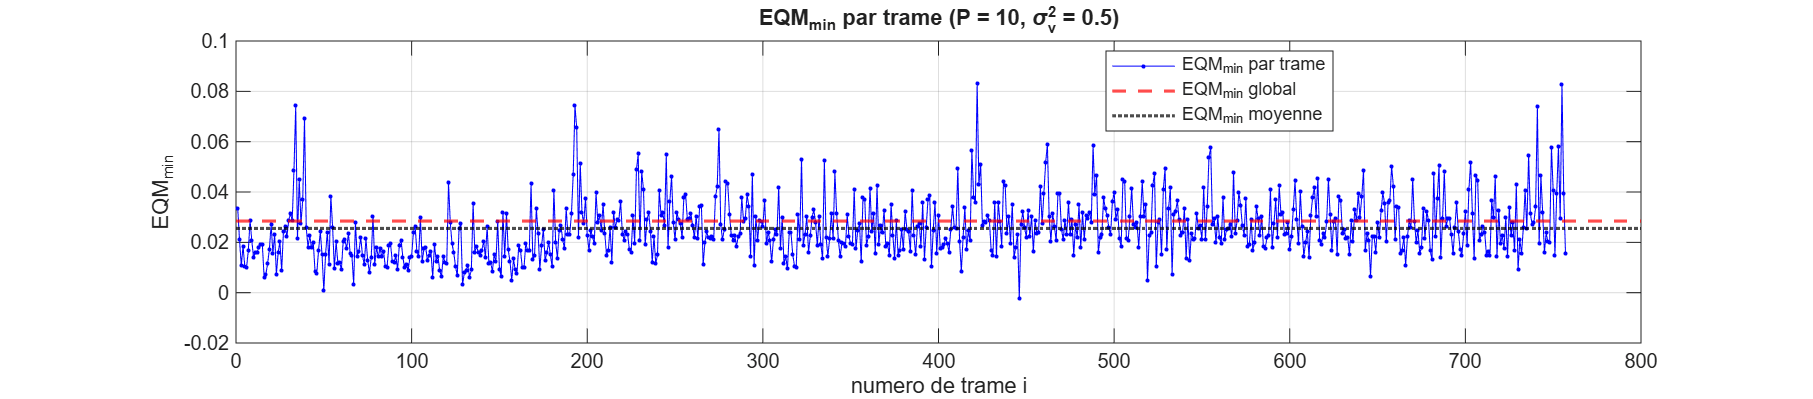
\includegraphics[width=\linewidth]{p3_qd_eqm_trames}
  \caption{$\mathrm{EQM}_{\min}$ de chaque trame, comparée à $\mathrm{EQM}_{\min}$ globale et à la moyenne des trames ($P=10$, $\sigma_v^2=0.5$).}
\end{figure}

\begin{figure}[H]
  \centering
  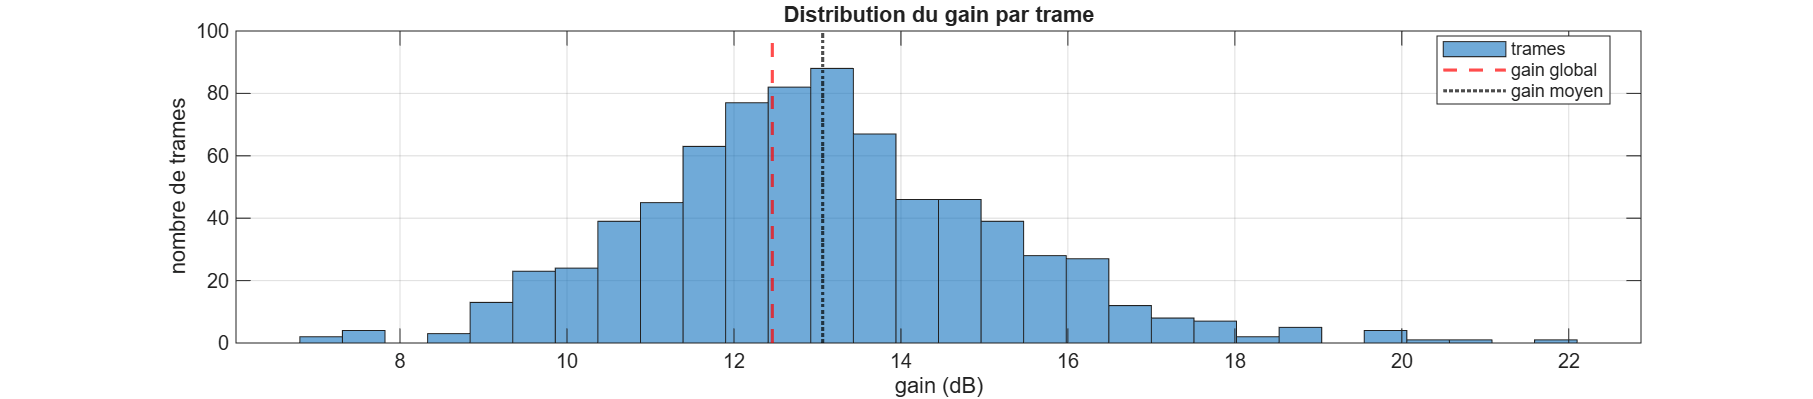
\includegraphics[width=\linewidth]{p3_qd_hist_gain}

  \medskip
  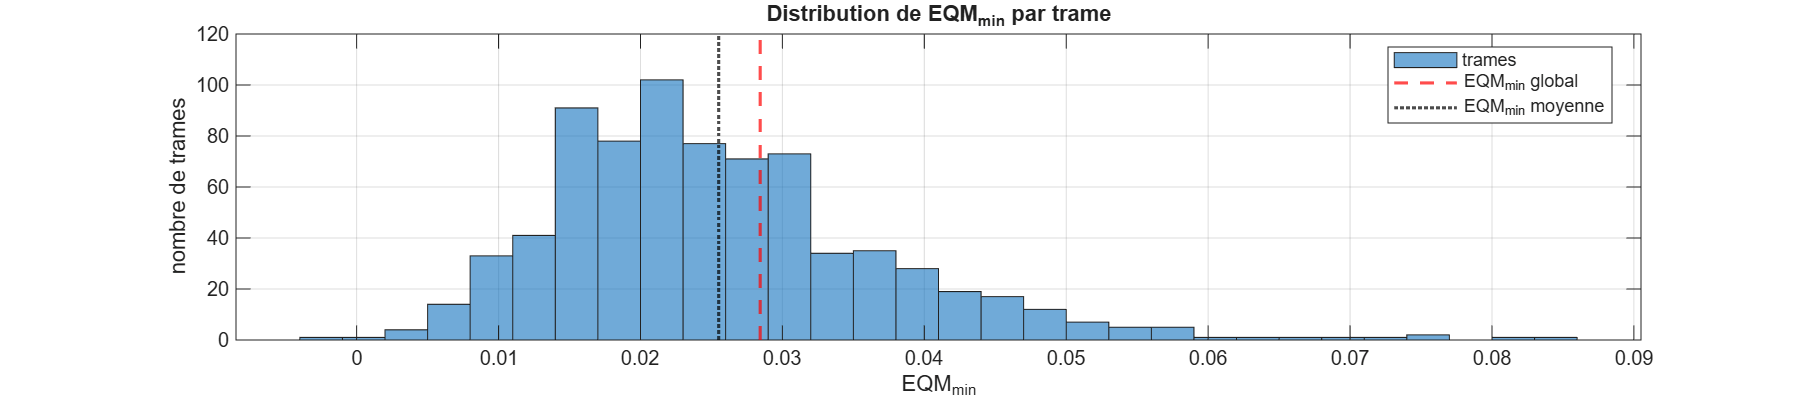
\includegraphics[width=\linewidth]{p3_qd_hist_eqm}
  \caption{Distributions du gain (en haut) et de $\mathrm{EQM}_{\min}$ (en bas) sur les $757$ trames (fonction \texttt{histogram}).}
\end{figure}

\begin{figure}[H]
  \centering
  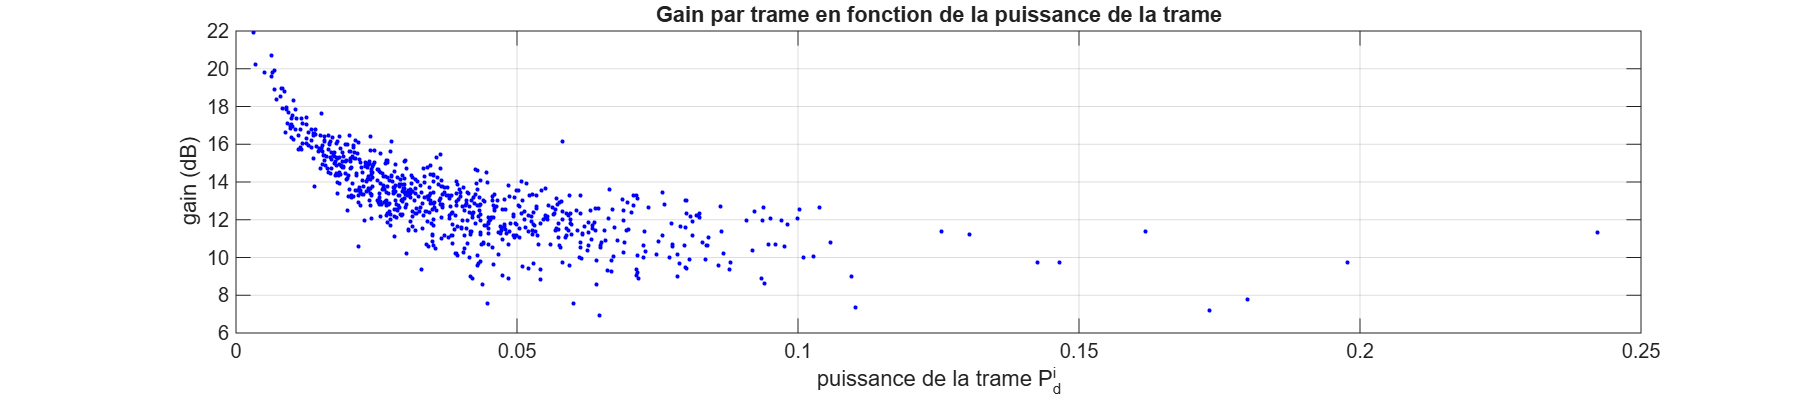
\includegraphics[width=\linewidth]{p3_qd_gain_vs_puissance}
  \caption{Gain de chaque trame en fonction de sa puissance $P^i_d$.}
\end{figure}

\begin{table}[H]
  \centering
  \begin{tabular}{lccccccc}
    \toprule
     & Moyenne & Écart-type & Médiane & Min & Max & $Q_1$ & $Q_3$ \\
    \midrule
    $\mathrm{gain}|_{\mathrm{dB}}$ (dB) & 13.06 & 2.14 & 12.94 & 6.92 & 21.90 & 11.66 & 14.34 \\
    $\mathrm{EQM}_{\min}$ & 0.0255 & 0.0118 & 0.0234 & $-0.0025$ & 0.0832 & 0.0171 & 0.0313 \\
    \bottomrule
  \end{tabular}
  \caption{Description statistique sur les $757$ trames. Sur tout le signal : $\mathrm{gain}|_{\mathrm{dB}}=12.46$~dB et $\mathrm{EQM}_{\min}=0.0284$.}
\end{table}

\begin{resultat}[Fonction MATLAB]
\texttt{histogram} (ou \texttt{hist}) pour la distribution, complétée par \texttt{mean}, \texttt{std}, \texttt{median}, \texttt{min}, \texttt{max} ; \texttt{boxplot} (Statistics Toolbox) résume médiane, quartiles et valeurs extrêmes en une figure.
\end{resultat}

\begin{interpretation}
\begin{itemize}
  \item \textbf{Comparaison au global.} $\mathrm{EQM}_{\min}$ moyenne des trames : $0.0255$, contre $0.0284$ sur tout le signal. Cohérent avec le gain moyen plus élevé trouvé en (c).
  \item \textbf{Distribution du gain.} En cloche, quasi symétrique : moyenne ($13.06$) $\approx$ médiane ($12.94$~dB). La moitié des trames est entre $11.66$ et $14.34$~dB, mais l'étendue est large ($6.92$ à $21.90$~dB), avec une petite queue vers les forts gains.
  \item \textbf{Distribution de $\mathrm{EQM}_{\min}$.} Dissymétrique, avec une queue vers les grandes valeurs (jusqu'à $0.083$) : moyenne $>$ médiane. Dispersion forte (écart-type $\approx$ moitié de la moyenne). Les $\approx 170$ premières trames ont une erreur plus faible ($0.01$--$0.02$).
  \item \textbf{Valeur négative.} Une trame donne $\mathrm{EQM}_{\min}=-0.0025$, physiquement impossible : c'est l'erreur d'estimation de la partie~2 ($r_{dx}=r_d$ supposé), fortement amplifiée par l'estimation sur $132$ échantillons.
  \item \textbf{Origine de la dispersion du gain.} Plus la trame est faible, plus le gain est élevé : $17$--$22$~dB pour $P^i_d<0.01$, $7$--$13$~dB pour $P^i_d>0.05$. Comme $\mathrm{gain}|_{\mathrm{dB}}=10\log_{10}(P_v/P_e)$ et que $P_e$ reste de l'ordre de $P^i_d$ au plus (le filtre atténue sa sortie quand le bruit domine), un fort gain signifie surtout que le bruit a été supprimé, pas que le signal est bien reconstruit. Les premières trames correspondent à un passage plus calme.
\end{itemize}
\end{interpretation}

\subsection{Question (e) : autocorrélation de référence calculée sur la trame 1}

\begin{enonce}
\textbf{Énoncé :} En supposant que l'autocorrélation du signal de référence a été calculée uniquement sur la trame n°1, réaliser le débruitage avec $\mathbf{w}^i_{opt}=(\mathbf{R}^i_x)^{-1}\mathbf{r}^1_{d}$. Comparer les performances par rapport aux deux démarches précédentes. Interpréter.
\end{enonce}

\textbf{Démarche.}
\begin{enumerate}
  \item Même découpage qu'en (c) ($K=757$, $L=132$, $P=10$, $\sigma_v^2=0.5$).
  \item Comparaison équitable : le bruit est généré \textbf{une seule fois}, les trois méthodes débruitent le même $x(n)$.
  \item $\mathbf{r}^1_{d}$ est calculé une fois sur la trame 1 ; pour chaque trame on estime $\mathbf{R}^i_x$ et on calcule les deux filtres $(\mathbf{R}^i_x)^{-1}\mathbf{r}^i_{d}$ (méthode (c)) et $(\mathbf{R}^i_x)^{-1}\mathbf{r}^1_{d}$ (méthode (e)).
  \item Chaque trame est filtrée avec ses $P-1$ échantillons précédents (pas de redémarrage à zéro).
  \item Critères : gain de chaque trame et gain $10\log_{10}(P_v/P_e)$ du signal \textbf{reconstruit}, plus fiable que la moyenne de gains en dB.
\end{enumerate}

\textbf{Code.}
\begin{lstlisting}
clear; clc; close all;
rng(0);
figDir = 'figs_partie3';

% Signal
[y, Fs] = audioread('monson.wav');
y = y(:,1);
N = 1e5;  debut = round(1*Fs);
d = y(debut+1 : debut+N);
d = d / max(abs(d));
P = 10;  sigv2 = 0.5;

% Decoupage en trames de 3 ms
L = round(3e-3 * Fs);
K = floor(N / L);
M = K*L;                             % echantillons couverts par les trames

% Bruit genere une seule fois : meme signal bruite pour les 3 methodes
v = sqrt(sigv2)*randn(N,1);
x = d + v;

% r_d calcule uniquement sur la trame 1
rd1 = xcorr(d(1:L), P-1, 'biased'); rd1 = rd1(P:end);

gain_i = zeros(K,1);                 % methode (c) : r_d de la trame i
gain_1 = zeros(K,1);                 % methode (e) : r_d de la trame 1
dhat_i = zeros(M,1);
dhat_1 = zeros(M,1);

for i = 1:K
    idx = (i-1)*L+1 : i*L;
    xi = x(idx);  di = d(idx);  vi = v(idx);

    % R_x et r_d de la trame i
    rx = xcorr(xi, P-1, 'biased'); rx = rx(P:end);
    Rx = toeplitz(rx);
    rdi = xcorr(di, P-1, 'biased'); rdi = rdi(P:end);

    % Les deux filtres
    h_i = Rx \ rdi;
    h_1 = Rx \ rd1;
    % Filtrage avec les P-1 echantillons precedents
    deb = max(1, idx(1) - (P-1));
    xe  = x(deb : idx(end));
    dh_i = filter(h_i, 1, xe);  dh_i = dh_i(end-L+1:end);
    dh_1 = filter(h_1, 1, xe);  dh_1 = dh_1(end-L+1:end);

    % Reconstruction
    dhat_i(idx) = dh_i;
    dhat_1(idx) = dh_1;

    % Gains de la trame
    Sv = 0; Se_i = 0; Se_1 = 0;
    for k = 1:L
        Sv   = Sv   + vi(k)^2;
        Se_i = Se_i + (di(k) - dh_i(k))^2;
        Se_1 = Se_1 + (di(k) - dh_1(k))^2;
    end
    gain_i(i) = 10*log10(Sv / Se_i);
    gain_1(i) = 10*log10(Sv / Se_1);
end

% Methode globale (un seul filtre pour tout le signal)
rx = xcorr(x, P-1, 'biased'); rx = rx(P:end);
rd = xcorr(d, P-1, 'biased'); rd = rd(P:end);
h_g = toeplitz(rx) \ rd;
dhat_g = filter(h_g, 1, x);

% Gain de chaque signal reconstruit
Sv = 0; Se_g = 0; Se_i = 0; Se_1 = 0;
for k = 1:M
    Sv   = Sv   + v(k)^2;
    Se_g = Se_g + (d(k) - dhat_g(k))^2;
    Se_i = Se_i + (d(k) - dhat_i(k))^2;
    Se_1 = Se_1 + (d(k) - dhat_1(k))^2;
end
G_g = 10*log10(Sv / Se_g);
G_i = 10*log10(Sv / Se_i);
G_1 = 10*log10(Sv / Se_1);

fprintf('global = %.2f | trames r_d^i = %.2f | trames r_d^1 = %.2f\n', ...
        G_g, G_i, G_1);
fprintf('r_d^i : moy = %.2f | med = %.2f | std = %.2f\n', ...
        mean(gain_i), median(gain_i), std(gain_i));
fprintf('r_d^1 : moy = %.2f | med = %.2f | std = %.2f\n', ...
        mean(gain_1), median(gain_1), std(gain_1));
fprintf('Trames ou r_d^1 fait mieux : %d / %d\n', sum(gain_1 > gain_i), K);

% Gain par trame avec r_d^1
figure;
plot(1:K, gain_1, 'm.-'); hold on;
yline(mean(gain_1), 'k:', 'LineWidth', 1.5);
yline(G_g, 'r--', 'LineWidth', 1.5);
grid on; xlabel('numero de trame i'); ylabel('gain (dB)');
legend('gain par trame (r_d^1)', 'gain moyen par trame', 'gain global', ...
       'Location', 'best');
drawnow;
exportgraphics(gcf, fullfile(figDir, 'p3_qe_gain_trames.png'), 'Resolution', 150);

% Comparaison des deux methodes par trame
figure;
plot(1:K, gain_i, 'b.-'); hold on;
plot(1:K, gain_1, 'm.-');
yline(G_g, 'r--', 'LineWidth', 1.5);
grid on; xlabel('numero de trame i'); ylabel('gain (dB)');
legend('r_d^i (question c)', 'r_d^1 (question e)', 'gain global', ...
       'Location', 'best');
drawnow;
exportgraphics(gcf, fullfile(figDir, 'p3_qe_comparaison.png'), 'Resolution', 150);

% Distributions des deux methodes
figure;
histogram(gain_i, 30, 'DisplayStyle', 'stairs', 'EdgeColor', 'b', 'LineWidth', 1.5); hold on;
histogram(gain_1, 30, 'DisplayStyle', 'stairs', 'EdgeColor', 'm', 'LineWidth', 1.5);
xline(G_g, 'r--', 'LineWidth', 1.5);
grid on; xlabel('gain (dB)'); ylabel('nombre de trames');
legend('r_d^i (question c)', 'r_d^1 (question e)', 'gain global', ...
       'Location', 'best');
drawnow;
exportgraphics(gcf, fullfile(figDir, 'p3_qe_hist.png'), 'Resolution', 150);

%% Ecoute (meme volume pour les trois)
soundsc(dhat_g, Fs);  pause(N/Fs + 0.5);
soundsc(dhat_i, Fs);  pause(N/Fs + 0.5);
soundsc(dhat_1, Fs);
\end{lstlisting}

\begin{figure}[H]
  \centering
  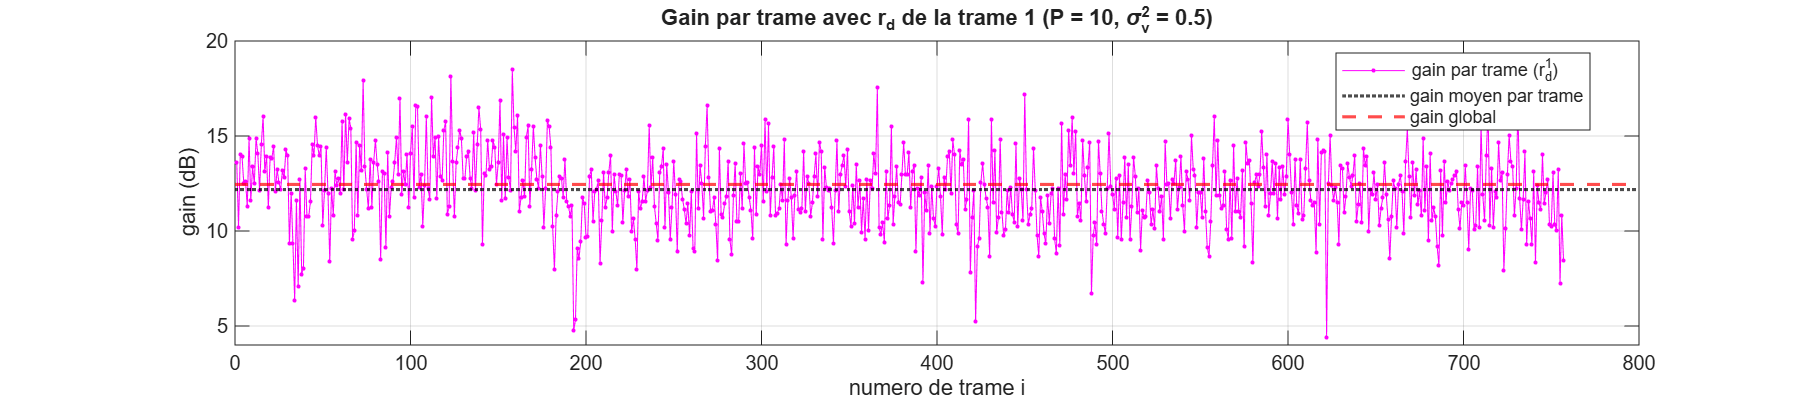
\includegraphics[width=\linewidth]{p3_qe_gain_trames}
  \caption{Gain par trame avec $\mathbf{r}^1_{d}$, comparé au gain moyen par trame et au gain global ($P=10$, $\sigma_v^2=0.5$).}
\end{figure}

\begin{figure}[H]
  \centering
  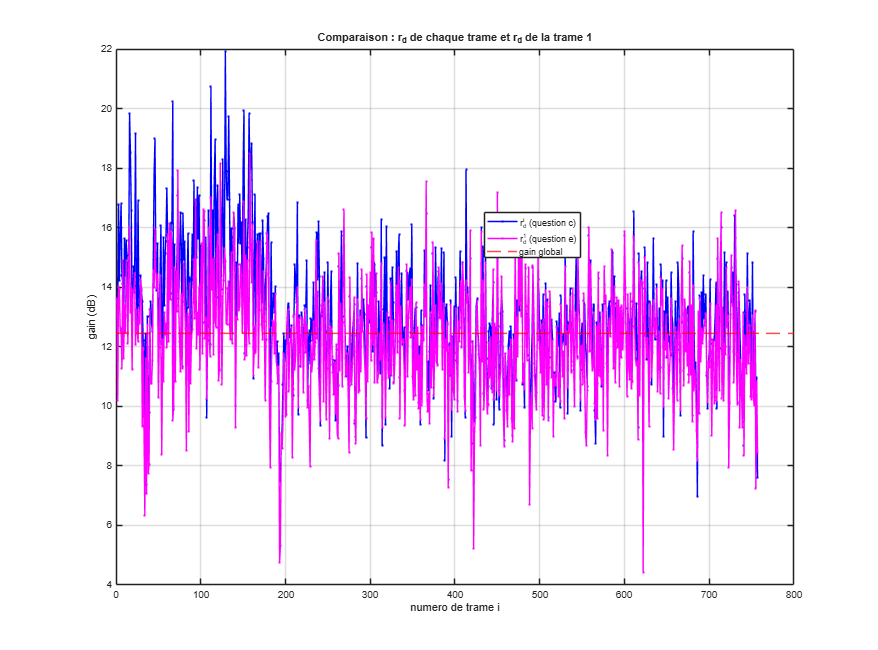
\includegraphics[width=0.85\linewidth]{p3_qe_comparaison}
  \caption{Gain par trame avec $\mathbf{r}^i_{d}$ (question c) et avec $\mathbf{r}^1_{d}$ (question e).}
\end{figure}

\begin{figure}[H]
  \centering
  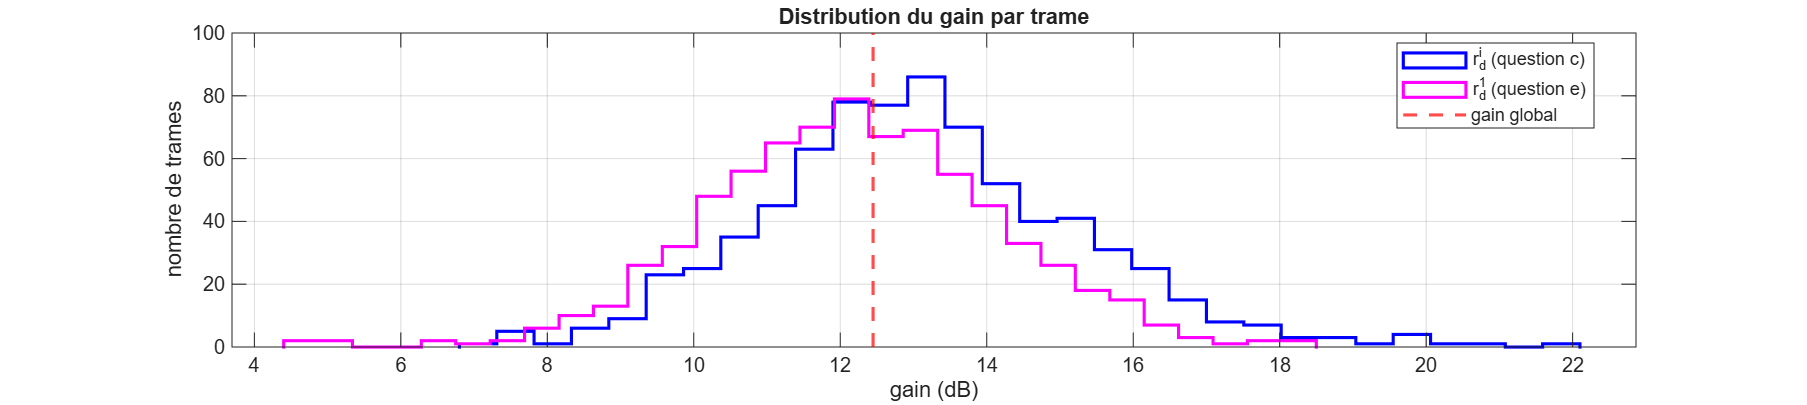
\includegraphics[width=\linewidth]{p3_qe_hist}
  \caption{Distribution du gain par trame pour les deux méthodes.}
\end{figure}

\begin{table}[H]
  \centering
  \begin{tabular}{lccc}
    \toprule
    Méthode & Filtre unique (global) & Trames, $\mathbf{r}^i_{d}$ (c) & Trames, $\mathbf{r}^1_{d}$ (e) \\
    \midrule
    Gain du signal reconstruit (dB) & 12.45 & 12.6 & 11.76 \\
    \bottomrule
  \end{tabular}
  \caption{Comparaison des trois démarches sur le même signal bruité ($P=10$, $\sigma_v^2=0.5$).}
\end{table}

\begin{resultat}
La méthode (e) est la moins bonne : $-0.9$~dB par rapport à (c) et $-0.7$~dB par rapport au filtre global. L'avantage réel de (c) sur le filtre global n'est que de $\approx 0.2$~dB (la moyenne des gains en dB annonçait $0.6$~dB).
\end{resultat}

\begin{interpretation}
\begin{itemize}
  \item \textbf{Par trame.} Avec $\mathbf{r}^1_{d}$, gain moyen $12.17$~dB et médiane $12.19$~dB (environ $13$~dB avec $\mathbf{r}^i_{d}$). Seules $166$ trames sur $757$ ($22\,\%$) font mieux qu'avec $\mathbf{r}^i_{d}$. L'histogramme est décalé d'environ $1$~dB vers la gauche : plus aucune trame au-delà de $18.5$~dB (contre $22$~dB), et des chutes jusqu'à $4.4$~dB (trames $\approx 35$, $193$, $420$, $622$). L'écart est surtout visible sur les $180$ premières trames.
  \item \textbf{Explication.} Utiliser $\mathbf{r}^1_{d}$ partout revient à supposer que le signal garde les statistiques de ses $3$ premières millisecondes : faux pour un signal non stationnaire. $\mathbf{R}^i_x$ et $\mathbf{r}^1_{d}$ décrivent alors deux portions différentes, et le filtre n'est plus optimal : il laisse passer trop de bruit si la trame $i$ est plus faible que la trame 1, et atténue trop si elle est plus forte. Le filtre global fait mieux car son autocorrélation est moyennée sur tout le signal, et non estimée sur $132$ échantillons.
  \item \textbf{Perte limitée} ($0.7$~dB) : $\mathbf{R}^i_x$ est toujours recalculée sur chaque trame, et les $10$ premiers retards de l'autocorrélation décrivent surtout le caractère passe-bas du signal, qui varie peu.
  \item \textbf{Intérêt pratique.} Ce cas est plus réaliste : on ne dispose en général du signal propre que sur une courte période d'apprentissage. Alternatives : estimer $r_d(k)=r_x(k)-\sigma_v^2\delta(k)$ à partir du signal bruité (testé en (f)), ou utiliser un filtre adaptatif LMS.
  \item \textbf{Écoute.} À volume égal, le débruitage global sonne mieux que les deux débruitages par trames, malgré un gain légèrement inférieur à (c) :
  \begin{itemize}
    \item \emph{clics toutes les 3~ms} dus au changement brusque des coefficients : saut moyen entre échantillons voisins de $0.065$ aux frontières contre $0.037$ ailleurs avec $\mathbf{r}^i_{d}$ ($0.069$ contre $0.044$ avec $\mathbf{r}^1_{d}$), contre $0.037$/$0.036$ pour le filtre global ; quelques filtres mal estimés produisent aussi des pics ($0.95$ contre $0.52$) ;
    \item \emph{plus de bruit résiduel} : $0.0104$ (et $0.0126$ avec $\mathbf{r}^1_{d}$) contre $0.0087$ pour le filtre global ; les trames réduisent l'EQM surtout en conservant plus de signal ($36\,\%$ contre $31\,\%$).
  \end{itemize}
  L'oreille étant plus sensible au bruit et aux clics qu'à une légère atténuation, le gain en RSB ne reflète pas la qualité perçue.
\end{itemize}
\end{interpretation}

\subsection{Question (f) : autres scénarios à étudier}

\begin{enonce}
\textbf{Énoncé :} Citer d'autres scénarios dont vous devez étudier les performances de ce type de débruitage.
\end{enonce}

\begin{resultat}[Scénarios à étudier]
\begin{enumerate}
  \item \textbf{Durée des trames} (compromis stationnarité / fiabilité des estimations / discontinuités) --- \emph{simulé ci-dessous}.
  \item \textbf{Signal propre indisponible} : $r_d(k)$ estimé à partir du signal bruité, $r_d(k)=r_x(k)-\sigma_v^2\delta(k)$ --- \emph{simulé}.
  \item \textbf{Niveau de bruit} (RSB d'entrée) --- \emph{simulé}.
  \item \textbf{Bruit coloré} (non blanc) --- \emph{simulé}.
  \item \textbf{Trames qui se chevauchent} avec fenêtre (Hanning) et reconstruction par addition-recouvrement, pour supprimer les clics.
  \item \textbf{$\sigma_v^2$ inconnue}, estimée sur un passage sans signal.
  \item \textbf{Bruit non stationnaire ou non gaussien} : impulsionnel, de puissance variable, bruit réel (rue, moteur, foule).
  \item \textbf{Autres signaux} : parole, musique, signaux biomédicaux.
  \item \textbf{Filtre adaptatif LMS} de Widrow, sans trames ni connaissance des statistiques.
  \item \textbf{Critères perceptifs} (PESQ, STOI) en complément du gain en RSB.
\end{enumerate}
\end{resultat}

\textbf{Démarche des simulations.} Même signal, $P=10$, \texttt{rng(0)}. Deux fonctions : \texttt{gain\_global} (un filtre sur tout le signal) et \texttt{gain\_trames} (un filtre par trame, avec les $P-1$ échantillons précédents). Les discontinuités sont mesurées par le rapport entre le saut moyen aux frontières des trames et le saut moyen ailleurs ($1$ = pas de discontinuité). Le bruit coloré est $v(n)=0.9\,v(n-1)+w(n)$, ramené à la même puissance que le bruit blanc.

\textbf{Code.}
\begin{lstlisting}
clear; clc; close all;
rng(0);
figDir = 'figs_partie3';

% Signal
[y, Fs] = audioread('monson.wav');
y = y(:,1);
N = 1e5;  debut = round(1*Fs);
d = y(debut+1 : debut+N);
d = d / max(abs(d));
P = 10;

%% Scenarios 1 et 2 : duree des trames et estimation de r_d
sigv2 = 0.5;
v = sqrt(sigv2)*randn(N,1);
x = d + v;

durees = [3 10 20 50 100];           % en ms
modes  = {'rdi', 'rd1', 'estime'};
nD = length(durees);  nM = length(modes);
G    = zeros(nD, nM);
saut = zeros(nD, nM);

G_glob = gain_global(d, x, v, P);
for k = 1:nD
    L = round(durees(k)*1e-3 * Fs);
    for m = 1:nM
        [G(k,m), saut(k,m)] = gain_trames(d, x, v, P, L, modes{m}, sigv2);
    end
    fprintf('trames %3d ms : r_d^i = %5.2f | r_d^1 = %5.2f | estime = %5.2f dB | global = %5.2f dB\n', ...
            durees(k), G(k,1), G(k,2), G(k,3), G_glob);
end
fprintf('saut frontieres / saut ailleurs (r_d^i) : %s\n', mat2str(saut(:,1)', 3));

% Gain en fonction de la duree des trames
figure;
plot(durees, G(:,1), 'b-o', 'LineWidth', 1.3); hold on;
plot(durees, G(:,2), 'm-s', 'LineWidth', 1.3);
plot(durees, G(:,3), 'g-^', 'LineWidth', 1.3);
yline(G_glob, 'r--', 'LineWidth', 1.5);
set(gca, 'XScale', 'log'); xticks(durees); grid on;
xlabel('duree des trames (ms)'); ylabel('gain du signal reconstruit (dB)');
legend('r_d^i (trame i)', 'r_d^1 (trame 1)', 'r_d estime depuis x', 'global', ...
       'Location', 'best');
drawnow;
exportgraphics(gcf, fullfile(figDir, 'p3_qf_gain_duree.png'), 'Resolution', 150);

% Discontinuites aux frontieres
figure;
plot(durees, saut(:,1), 'b-o', 'LineWidth', 1.3); hold on;
plot(durees, saut(:,2), 'm-s', 'LineWidth', 1.3);
plot(durees, saut(:,3), 'g-^', 'LineWidth', 1.3);
yline(1, 'k:', 'LineWidth', 1.5);
set(gca, 'XScale', 'log'); xticks(durees); grid on;
xlabel('duree des trames (ms)'); ylabel('saut frontieres / saut ailleurs');
legend('r_d^i (trame i)', 'r_d^1 (trame 1)', 'r_d estime depuis x', ...
       'sans discontinuite', 'Location', 'best');
drawnow;
exportgraphics(gcf, fullfile(figDir, 'p3_qf_saut_duree.png'), 'Resolution', 150);

%% Scenario 3a : niveau de bruit (trames de 20 ms)
sigList = [0.05 0.1 0.5 1];
nS  = length(sigList);
L20 = round(20e-3 * Fs);
Gs = zeros(nS, 3);  RSBav = zeros(nS, 1);
for s = 1:nS
    vs = sqrt(sigList(s))*randn(N,1);
    xs = d + vs;
    RSBav(s) = 10*log10(mean(d.^2) / sigList(s));
    Gs(s,1) = gain_global(d, xs, vs, P);
    Gs(s,2) = gain_trames(d, xs, vs, P, L20, 'rdi', sigList(s));
    Gs(s,3) = gain_trames(d, xs, vs, P, L20, 'estime', sigList(s));
    fprintf('sigv2 = %.2f (RSB_av = %5.2f dB) : global = %5.2f | r_d^i = %5.2f | estime = %5.2f dB\n', ...
            sigList(s), RSBav(s), Gs(s,1), Gs(s,2), Gs(s,3));
end

figure;
plot(RSBav, Gs(:,1), 'r-o', 'LineWidth', 1.3); hold on;
plot(RSBav, Gs(:,2), 'b-s', 'LineWidth', 1.3);
plot(RSBav, Gs(:,3), 'g-^', 'LineWidth', 1.3);
grid on; xlabel('RSB avant debruitage (dB)'); ylabel('gain (dB)');
legend('global', 'trames r_d^i', 'trames r_d estime', 'Location', 'best');
drawnow;
exportgraphics(gcf, fullfile(figDir, 'p3_qf_gain_bruit.png'), 'Resolution', 150);

%% Scenario 3b : bruit blanc ou bruit colore (meme puissance)
sigv2 = 0.5;
vb = sqrt(sigv2)*randn(N,1);              % bruit blanc
vc = filter(1, [1 -0.9], randn(N,1));     % bruit colore passe-bas
vc = vc * sqrt(sigv2 / mean(vc.^2));      % meme puissance que vb
Plist = 5:5:50;
Gb = zeros(size(Plist));  Gc = zeros(size(Plist));
for m = 1:length(Plist)
    Gb(m) = gain_global(d, d + vb, vb, Plist(m));
    Gc(m) = gain_global(d, d + vc, vc, Plist(m));
end
fprintf('P = 10 : bruit blanc = %.2f dB | bruit colore = %.2f dB\n', Gb(2), Gc(2));

figure;
plot(Plist, Gb, 'b-o', 'LineWidth', 1.3); hold on;
plot(Plist, Gc, 'r-s', 'LineWidth', 1.3);
grid on; xticks(Plist);
xlabel('Ordre P'); ylabel('gain (dB)');
legend('bruit blanc', 'bruit colore (passe-bas)', 'Location', 'best');
drawnow;
exportgraphics(gcf, fullfile(figDir, 'p3_qf_bruit_colore.png'), 'Resolution', 150);

%% Ecoute : trames de 3 ms puis de 20 ms (meme echelle)
L3 = round(3e-3 * Fs);
[~, ~, dh3]  = gain_trames(d, x, v, P, L3,  'rdi', 0.5);
[~, ~, dh20] = gain_trames(d, x, v, P, L20, 'rdi', 0.5);
sc = max(abs([dh3; dh20]));
sound(dh3/sc, Fs);   pause(length(dh3)/Fs + 0.5);
sound(dh20/sc, Fs);

%% ================= Fonctions =================
function G = gain_global(d, x, v, P)
% Gain du filtre de Wiener calcule sur tout le signal
rx = xcorr(x, P-1, 'biased'); rx = rx(P:end);
rd = xcorr(d, P-1, 'biased'); rd = rd(P:end);
h  = toeplitz(rx) \ rd;
dh = filter(h, 1, x);
Sv = 0; Se = 0;
for k = 1:length(d)
    Sv = Sv + v(k)^2;
    Se = Se + (d(k) - dh(k))^2;
end
G = 10*log10(Sv / Se);
end

function [G, saut, dh] = gain_trames(d, x, v, P, L, mode, sigv2)
% Debruitage par trames de L echantillons
% mode : 'rdi' (r_d de la trame i), 'rd1' (r_d de la trame 1),
%        'estime' (r_d = r_x - sigv2*delta, sans le signal propre)
K = floor(length(d) / L);  M = K*L;
dh  = zeros(M,1);
rd1 = xcorr(d(1:L), P-1, 'biased'); rd1 = rd1(P:end);
for i = 1:K
    idx = (i-1)*L+1 : i*L;
    rx = xcorr(x(idx), P-1, 'biased'); rx = rx(P:end);
    switch mode
        case 'rdi'
            rd = xcorr(d(idx), P-1, 'biased'); rd = rd(P:end);
        case 'rd1'
            rd = rd1;
        case 'estime'
            rd = rx;  rd(1) = rd(1) - sigv2;
    end
    h = toeplitz(rx) \ rd;
    deb = max(1, idx(1) - (P-1));            % P-1 echantillons precedents
    ye  = filter(h, 1, x(deb:idx(end)));
    dh(idx) = ye(end-L+1:end);
end
Sv = 0; Se = 0;
for k = 1:M
    Sv = Sv + v(k)^2;
    Se = Se + (d(k) - dh(k))^2;
end
G = 10*log10(Sv / Se);
df = abs(diff(dh));
saut = mean(df(L:L:end)) / mean(df);   % 1 = pas de discontinuite
end
\end{lstlisting}

\begin{figure}[H]
  \centering
  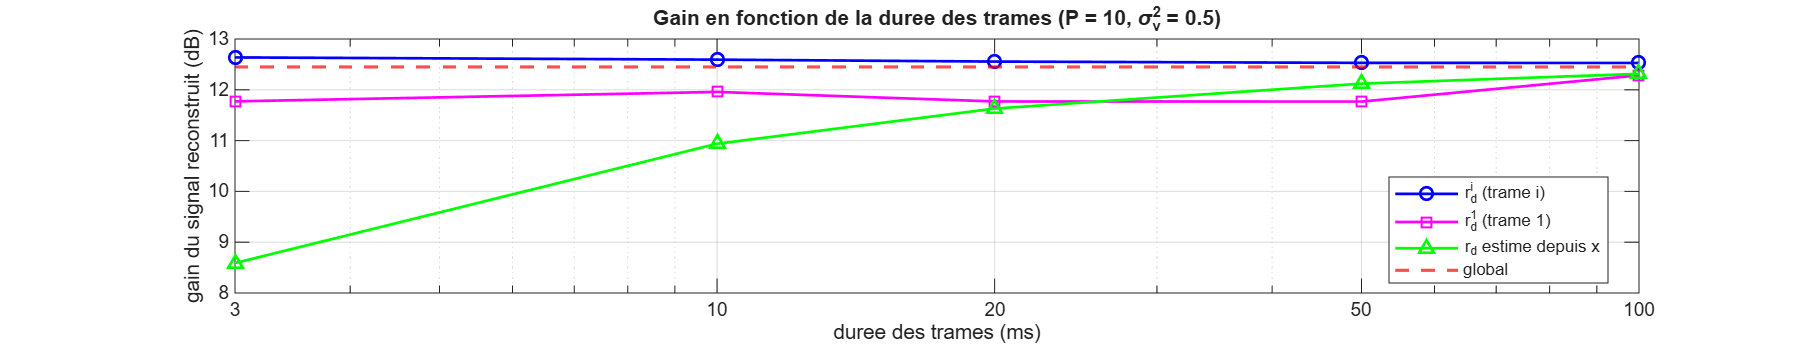
\includegraphics[width=\linewidth]{p3_qf_gain_duree}

  \medskip
  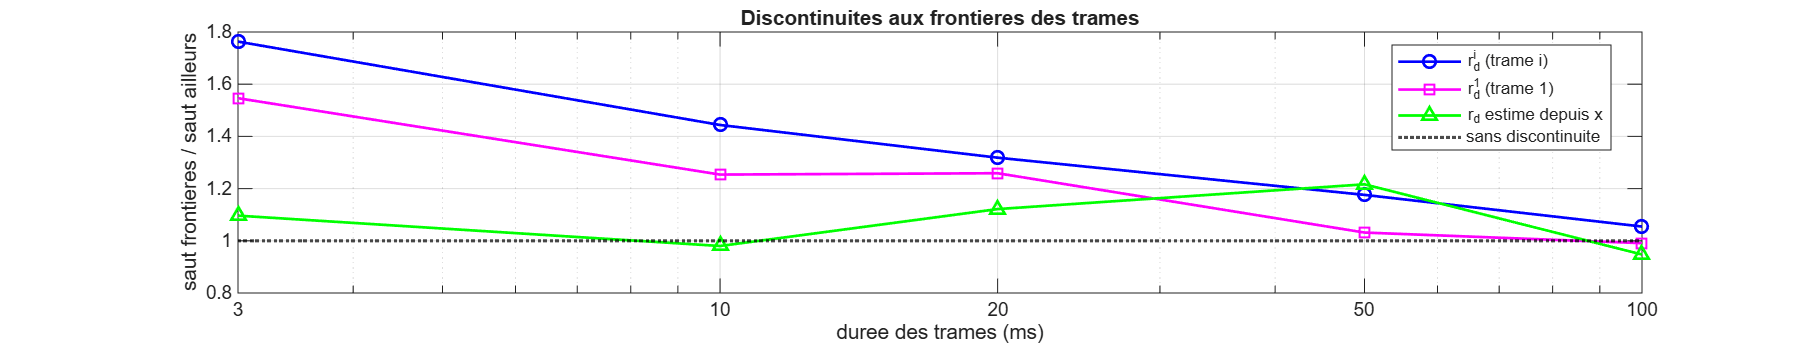
\includegraphics[width=\linewidth]{p3_qf_saut_duree}
  \caption{En haut : gain du signal reconstruit en fonction de la durée des trames, pour les trois façons d'obtenir $\mathbf{r}_{d}$. En bas : rapport saut aux frontières / saut ailleurs ($P=10$, $\sigma_v^2=0.5$).}
\end{figure}

\begin{figure}[H]
  \centering
  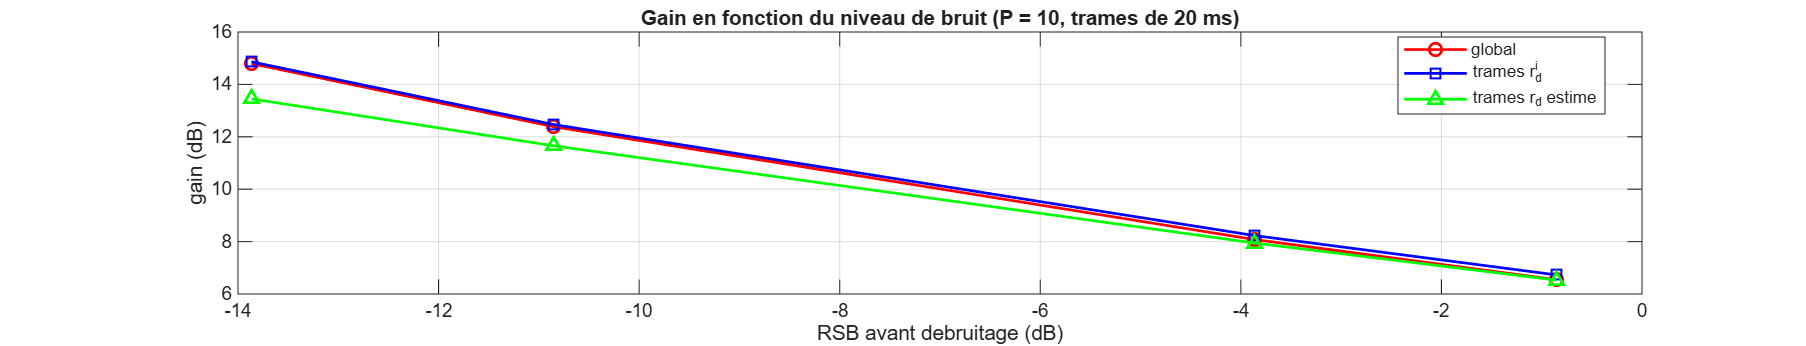
\includegraphics[width=\linewidth]{p3_qf_gain_bruit}

  \medskip
  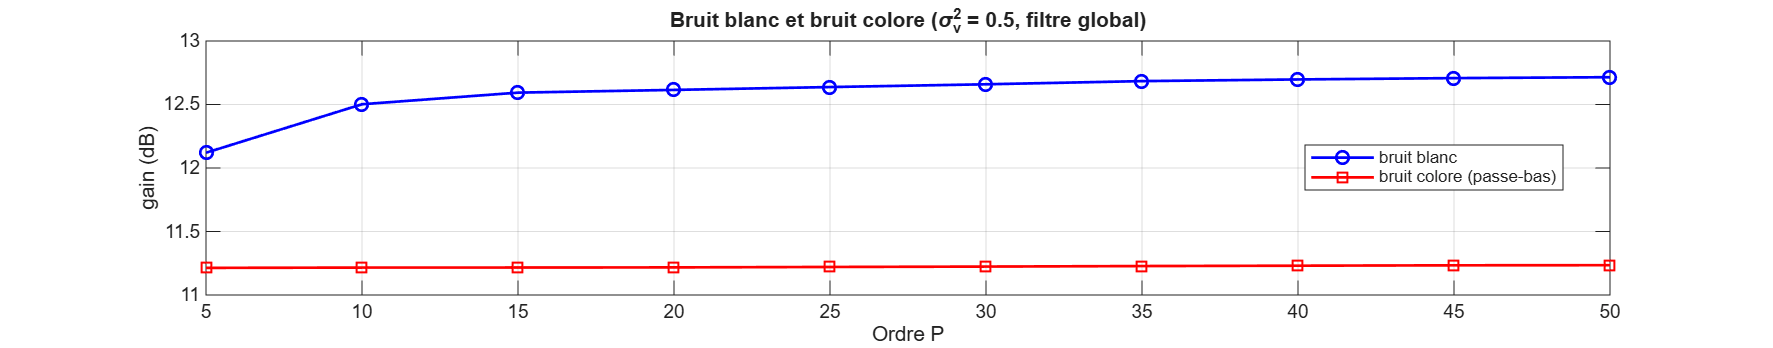
\includegraphics[width=\linewidth]{p3_qf_bruit_colore}
  \caption{En haut : gain en fonction du RSB avant débruitage ($P=10$, trames de $20$~ms). En bas : gain du filtre global en fonction de $P$ pour un bruit blanc et un bruit coloré de même puissance ($\sigma_v^2=0.5$).}
\end{figure}

\begin{interpretation}
\begin{itemize}
  \item \textbf{Durée des trames.} Avec $\mathbf{r}^i_{d}$, le gain ne dépend presque pas de la durée ($12.6$~dB à $3$~ms, $12.53$~dB à $100$~ms, toujours au-dessus du global : $12.45$~dB), mais les discontinuités diminuent nettement (rapport $1.76$ à $3$~ms, $1.32$ à $20$~ms, $1.05$ à $100$~ms). À l'écoute, les trames de $20$~ms sonnent nettement mieux que celles de $3$~ms : $6.7$ fois moins de frontières, des sauts plus faibles et des filtres estimés sur $882$ échantillons au lieu de $132$. Avec $\mathbf{r}^1_{d}$, le gain reste vers $11.8$~dB et ne remonte qu'à $100$~ms ($12.28$~dB), quand la trame 1 devient représentative.
  \item \textbf{Signal propre indisponible.} L'estimation $r_d(k)=r_x(k)-\sigma_v^2\delta(k)$ dépend fortement de la durée des trames : $8.59$~dB à $3$~ms, $11.63$~dB à $20$~ms, $12.31$~dB à $100$~ms (presque le global). Sur une trame courte, l'erreur d'estimation de $r_x(k)$ est amplifiée par la soustraction de $\sigma_v^2$. Compromis retenu : trames de $20$ à $50$~ms.
  \item \textbf{Niveau de bruit.} Le gain croît avec le bruit : $6.55$~dB pour $\sigma_v^2=0.05$ ($\mathrm{RSB}_{\mathrm{av}}=-0.86$~dB) à $14.79$~dB pour $\sigma_v^2=1$ ($\mathrm{RSB}_{\mathrm{av}}=-13.87$~dB), effet mécanique déjà vu en (c) et (d). Les trames avec $\mathbf{r}^i_{d}$ gardent $0.1$ à $0.2$~dB d'avance sur le global ; l'estimation sans signal propre perd jusqu'à $1.3$~dB à fort bruit.
  \item \textbf{Bruit coloré.} Pour $P=10$, le gain passe de $12.50$~dB (bruit blanc) à $11.22$~dB (bruit coloré), et augmenter $P$ n'apporte plus rien (courbe plate vers $11.2$~dB, contre $12.7$~dB en bruit blanc). Le bruit passe-bas occupe la même bande que le signal (les vagues) : un filtre linéaire ne peut pas séparer deux composantes de même bande, quel que soit son ordre.
\end{itemize}
\end{interpretation}

%==================== PARTIE 4 ====================
\section{Partie 4 : Séparation de deux voix par filtrage de Wiener}

\begin{enonce}
\textbf{Énoncé :} Implémenter un filtrage de Wiener sur le mélange $x=d_1+d_2$ pour séparer les deux sources, sur tout le signal puis par trame. Étudier l'effet de l'ordre $P$, de la longueur de trame et du recouvrement. Tracer les performances ($\mathrm{EQM}_{\min,j}$, gain en RSB, qualité perceptuelle PESQ), étudier la robustesse du filtre à la connaissance de $\mathbf{r}_{d_1}$ et envisager d'autres structures (cascade, soustraction, filtrage fréquentiel).
\end{enonce}

\textbf{Le problème.} Dans les parties 2 et 3, le signal à éliminer était un bruit blanc : il occupe toute la bande et ne ressemble pas au signal utile. Ici, le « bruit » est une seconde voix : il est coloré, non stationnaire et occupe la même bande que la voix recherchée. C'est le cas défavorable observé en partie~3~(f) avec le bruit coloré.

\textbf{Formulation.} On calcule un filtre par source. Pour extraire $d_j$ ($j=1,2$) :
\[
\mathbf{R}_x\,\mathbf{w}_j=\mathbf{r}_{d_jx},\qquad \hat d_j(n)=\sum_{k=0}^{P-1}w_j(k)\,x(n-k).
\]
Les deux voix sont indépendantes, donc décorrélées : $r_{d_jx}(k)=r_{d_j}(k)$ et $r_x(k)=r_{d_1}(k)+r_{d_2}(k)$. Dans le domaine fréquentiel (filtre de Wiener RII du cours), le filtre optimal vaut
\[
H_j(e^{j\omega})=\frac{P_{d_jx}(e^{j\omega})}{P_x(e^{j\omega})}=\frac{P_{d_j}(e^{j\omega})}{P_{d_1}(e^{j\omega})+P_{d_2}(e^{j\omega})}.
\]
À chaque fréquence, le filtre garde la part de la puissance qui appartient à $d_j$. Il ne peut donc séparer les voix que là où leurs spectres diffèrent.

\textbf{Critères.} Pour chaque source, $\mathrm{EQM}_{\min,j}=r_{d_j}(0)-\mathbf{w}_j^T\mathbf{r}_{d_j}$ et
\[
\mathrm{gain}_j|_{\mathrm{dB}}=10\log_{10}\frac{P_{d_j}}{\mathrm{EQM}_j}-10\log_{10}\frac{P_{d_j}}{P_{d_{j'}}},
\]
où $d_{j'}$ est l'autre voix, qui joue le rôle du bruit.

\textbf{Signaux.} Deux phrases de l'Open Speech Repository~\cite{osr} : une voix d'homme ($d_1$, \texttt{OSR\_us\_000\_0030\_8k.wav}) et une voix de femme ($d_2$, \texttt{OSR\_us\_000\_0010\_8k.wav}), échantillonnées à $F_s=8$~kHz. On garde les $8$ premières secondes ($N=64\,000$), on centre les signaux et on met $d_2$ à la puissance de $d_1$ : le RSB avant séparation vaut $0$~dB pour chaque source. Ce corpus est conçu pour les tests de qualité de la parole, et $8$~kHz est la fréquence de PESQ en bande étroite. Un mélange homme-femme est un cas favorable : les spectres des deux voix diffèrent.

\textbf{Organisation.}
\begin{itemize}
  \item Filtre global : mise en place, cas de référence.
  \item Ordre $P$, traitement par trames, recouvrement de 50~\% : suivre la non-stationnarité de la parole.
  \item Qualité perceptuelle (PESQ) : le RSB ne mesure pas ce que l'on entend.
  \item Robustesse à la connaissance de $\mathbf{r}_{d_1}$ (dictionnaire par $k$-means), puis proposition originale : filtre de Wiener itératif à modèle AR.
  \item Autres structures : cascade, soustraction, filtrage dans le domaine fréquentiel.
\end{itemize}

\subsection{Filtre global : mise en place et premiers résultats}

\begin{enonce}
\textbf{Objectif :} Calculer un seul filtre de Wiener par source sur tout le signal ($P=10$). C'est le cas de référence de la partie : on observe ce que le filtre exploite (les spectres des deux voix) et ce qu'il obtient.
\end{enonce}

\textbf{Démarche.} La fonction \texttt{separation\_wf} reprend le calcul de la partie~3 avec $d_j$ comme signal de référence et l'autre voix comme bruit. Elle est appelée deux fois, une fois par source. On trace les DSP des deux voix (\texttt{pwelch}) et les réponses en fréquence des deux filtres (\texttt{freqz}).

\textbf{Code.} Fonction de séparation :
\begin{lstlisting}
function [dhat, EQMmin, EQMmes, gain_dB, w] = separation_wf(x, d, b, P)
% Estimation de la source d dans le melange x = d + b par filtre de Wiener
% Entrees : x (melange), d (source cible), b (autre source), P (ordre)
% Sorties : dhat (source estimee), EQM theorique et mesuree, gain en dB, w

x = x(:); d = d(:); b = b(:);

rx = xcorr(x, P-1, 'biased'); rx = rx(P:end);
rd = xcorr(d, P-1, 'biased'); rd = rd(P:end);   % r_dx = r_d (sources decorrelees)
w  = toeplitz(rx) \ rd;              % filtre de Wiener
dhat = filter(w, 1, x);              % source estimee

EQMmin = rd(1) - w'*rd;              % EQM theorique
EQMmes = mean((d - dhat).^2);        % EQM mesuree

% Gain : RSB avant (d face a b) / RSB apres (d face au residu)
RSB_av  = 10*log10(mean(d.^2) / mean(b.^2));
RSB_ap  = 10*log10(mean(d.^2) / EQMmes);
gain_dB = RSB_ap - RSB_av;
end
\end{lstlisting}

Script principal :
\begin{lstlisting}
clear; clc; close all;
dossier = fileparts(mfilename('fullpath'));   % dossier du script
rep = fullfile(dossier, 'figs_partie4', filesep);
if ~isfolder(rep), mkdir(rep); end

%% Chargement des deux voix (Open Speech Repository, 8 kHz)
url = 'https://www.voiptroubleshooter.com/open_speech/american/';
f1  = fullfile(dossier, 'OSR_us_000_0030_8k.wav');   % voix d'homme
f2  = fullfile(dossier, 'OSR_us_000_0010_8k.wav');   % voix de femme
if ~isfile(f1), websave(f1, [url 'OSR_us_000_0030_8k.wav']); end
if ~isfile(f2), websave(f2, [url 'OSR_us_000_0010_8k.wav']); end
[d1, Fs1] = audioread(f1);
[d2, Fs2] = audioread(f2);
d1 = d1(:,1);  d2 = d2(:,1);
if Fs1 ~= Fs2                        % meme frequence d'echantillonnage
    d2 = resample(d2, Fs1, Fs2);
end
Fs = Fs1;

Tmax = 8;                            % duree gardee (s)
N  = min([length(d1), length(d2), round(Tmax*Fs)]);
d1 = d1(1:N);  d2 = d2(1:N);
d1 = d1 - mean(d1);  d2 = d2 - mean(d2);       % sources centrees
d2 = d2 * sqrt(mean(d1.^2) / mean(d2.^2));     % meme puissance -> RSB = 0 dB
x  = d1 + d2;                        % melange

%% Spectres des deux sources
[S1, f] = pwelch(d1, hamming(512), 256, 1024, Fs);
S2      = pwelch(d2, hamming(512), 256, 1024, Fs);
figure;
plot(f, 10*log10(S1), 'b', 'LineWidth', 1.2); hold on;
plot(f, 10*log10(S2), 'r', 'LineWidth', 1.2);
grid on; xlabel('f (Hz)'); ylabel('DSP (dB/Hz)');
legend('d_1 : voix d''homme', 'd_2 : voix de femme');
saveas(gcf, [rep 'p4_q1_dsp.png']);

%% Filtre de Wiener global
P = 10;
[d1h, EQM1, EQMm1, g1, w1] = separation_wf(x, d1, d2, P);
[d2h, EQM2, EQMm2, g2, w2] = separation_wf(x, d2, d1, P);

%% Reponses en frequence des deux filtres
[H1, fh] = freqz(w1, 1, 1024, Fs);
H2       = freqz(w2, 1, 1024, Fs);
figure;
plot(fh, abs(H1), 'b', 'LineWidth', 1.2); hold on;
plot(fh, abs(H2), 'r', 'LineWidth', 1.2);
plot(fh, abs(H1 + H2), 'k--');
grid on; xlabel('f (Hz)'); ylabel('|H(f)|');
legend('|H_1| : extrait d_1', '|H_2| : extrait d_2', '|H_1 + H_2|');
saveas(gcf, [rep 'p4_q1_freqz.png']);

%% Ecoute : melange, puis estimees
sound(x, Fs);    pause(N/Fs + 0.5);
sound(d1h, Fs);  pause(N/Fs + 0.5);
sound(d2h, Fs);
\end{lstlisting}

\begin{figure}[H]
  \centering
  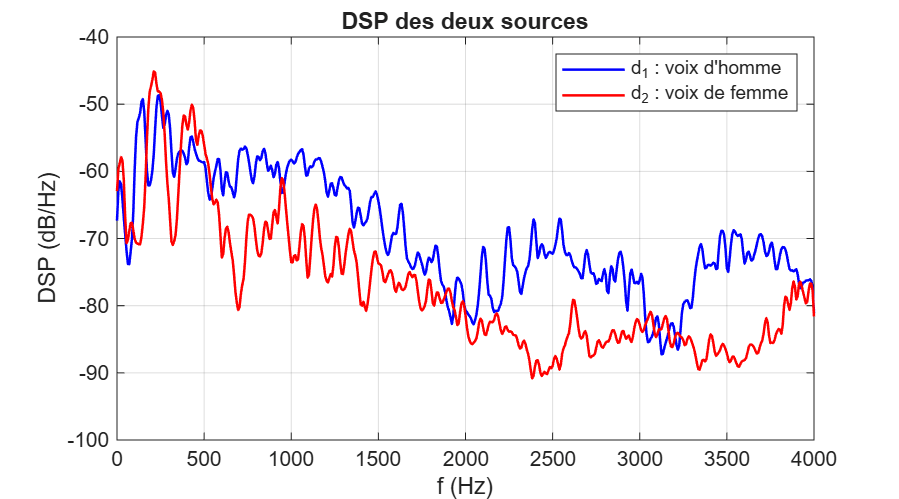
\includegraphics[width=\linewidth]{p4_q1_dsp}
  \caption{DSP de la voix d'homme $d_1$ et de la voix de femme $d_2$ (même puissance).}
\end{figure}

\begin{figure}[H]
  \centering
  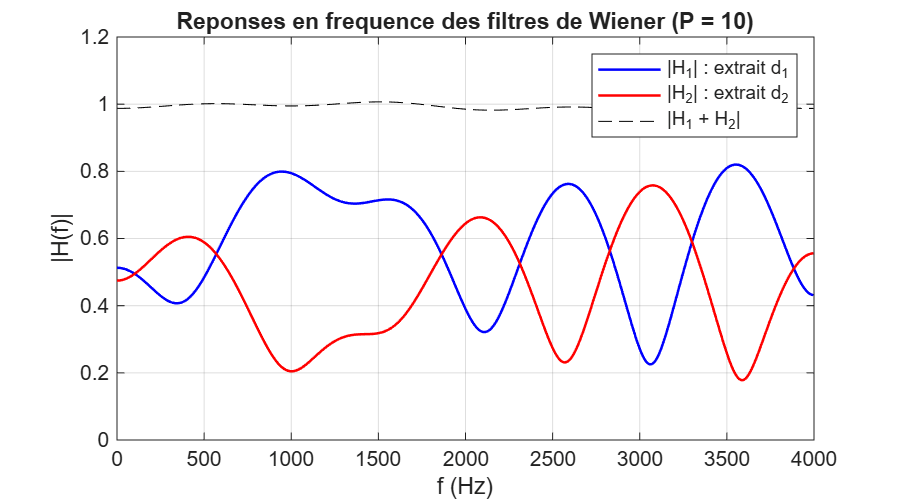
\includegraphics[width=\linewidth]{p4_q1_freqz}
  \caption{Réponses en fréquence des filtres de Wiener globaux ($P=10$) et de leur somme.}
\end{figure}

\begin{resultat}
$P_{d_1}=P_{d_2}=0.0027$. Pour les deux sources : $\mathrm{EQM}_{\min}=\mathrm{EQM}_{\text{mesurée}}=0.0012$, soit un gain de $\mathbf{3.48}$~dB (RSB de $0$ à $3.48$~dB).
\end{resultat}

\begin{interpretation}
\begin{itemize}
  \item \textbf{Qui domine où.} Le filtre ne dépend pas de l'endroit où chaque voix a le plus d'énergie, mais du rapport $P_{d_1}/P_{d_2}$ à chaque fréquence. L'homme domine sous $180$~Hz (son fondamental, entre $100$ et $150$~Hz) et au-dessus de $600$~Hz. La femme domine de $200$ à $500$~Hz, où se trouvent son fondamental ($\approx 200$~Hz) et sa 2\textsuperscript{e} harmonique : à puissance totale égale, elle concentre son énergie sur peu d'harmoniques.
  \item \textbf{Réponses des filtres.} $|H_1|$ est grand là où l'homme domine ($\approx 0.8$ vers $1$~kHz), $|H_2|$ là où la femme domine ($\approx 0.6$ vers $400$~Hz). Les gains restent entre $0.2$ et $0.8$ : le filtre ne coupe aucune fréquence, il pondère. Avec $P=10$ coefficients, sa résolution est grossière ($\approx F_s/P=800$~Hz) : il ne distingue pas la zone de l'homme sous $180$~Hz de celle de la femme entre $200$ et $500$~Hz.
  \item \textbf{$|H_1+H_2|\approx 1$, d'où des gains égaux.} Comme $\mathbf{r}_x=\mathbf{r}_{d_1}+\mathbf{r}_{d_2}$, on a $\mathbf{w}_1+\mathbf{w}_2=\mathbf{R}_x^{-1}\mathbf{r}_x=[1,0,\dots,0]^T$ ($\mathbf{r}_x$ est la première colonne de $\mathbf{R}_x$). Donc $\hat d_1+\hat d_2\approx x$ et $e_2\approx-e_1$ : les deux EQM sont égales, et les gains aussi puisque $P_{d_1}=P_{d_2}$. L'écart à $1$ ($<2$~\%) vient de l'intercorrélation de $d_1$ et $d_2$, non nulle sur une durée finie.
  \item \textbf{Écoute.} Dans $\hat d_1$, l'homme est nettement mis en avant ; dans $\hat d_2$, on entend peu de différence avec le mélange, pour le même gain en RSB. Le résidu d'homme dans $\hat d_2$ se trouve entre $600$ et $4000$~Hz, la zone où l'oreille est la plus sensible (formants, consonnes). Le RSB mesure une puissance d'erreur, pas ce que l'on entend : il faut une mesure perceptuelle comme PESQ.
\end{itemize}
\end{interpretation}

\begin{resultat}[Conclusion]
Le filtre global ne sépare que partiellement les deux voix ($+3.5$~dB) : il ne voit que les spectres moyens sur $8$~s, qui se recouvrent, et $P=10$ est trop faible pour suivre leurs détails. On étudie donc ensuite l'ordre $P$, le traitement par trames et l'évaluation par PESQ.
\end{resultat}

\subsection{Influence de l'ordre \texorpdfstring{$P$}{P} du filtre global}

\begin{enonce}
\textbf{Objectif :} Vérifier si un filtre plus long sépare mieux les deux voix. Avec $P$ coefficients, $H(f)$ ne peut pas former de détail plus étroit qu'environ $F_s/P$ : $800$~Hz pour $P=10$, $160$~Hz pour $P=50$, $40$~Hz pour $P=200$.
\end{enonce}

\textbf{Démarche.} Filtre global (tout le signal, $N=64\,000$), $P$ de $2$ à $200$. Le chargement des voix est regroupé dans une fonction \texttt{charger\_voix(Tmax)} (même code qu'en section précédente).

\textbf{Code.}
\begin{lstlisting}
[d1, d2, x, Fs] = charger_voix(8);

%% Gain du filtre global en fonction de P
Plist = [2 5 10 20 30 50 75 100 150 200];
g1 = zeros(size(Plist));  g2 = zeros(size(Plist));
for m = 1:length(Plist)
    P = Plist(m);
    [~, ~, ~, g1(m)] = separation_wf(x, d1, d2, P);
    [~, ~, ~, g2(m)] = separation_wf(x, d2, d1, P);
end
figure;
plot(Plist, g1, 'bo-', 'LineWidth', 1.3); hold on;
plot(Plist, g2, 'r*--', 'LineWidth', 1.1);
grid on; xlabel('P'); ylabel('gain (dB)');
legend('d_1 : homme', 'd_2 : femme', 'Location', 'southeast');
saveas(gcf, [rep 'p4_q2_gain_P.png']);

%% Reponse en frequence de H1 pour plusieurs P (resolution ~ Fs/P)
Pvis = [10 50 200];
coul = {'b', 'm', 'k'};
figure;
for m = 1:length(Pvis)
    [~, ~, ~, ~, w1] = separation_wf(x, d1, d2, Pvis(m));
    [H1, fh] = freqz(w1, 1, 2048, Fs);
    plot(fh, abs(H1), coul{m}, 'LineWidth', 1.1); hold on;
end
grid on; xlabel('f (Hz)'); ylabel('|H_1(f)|');
legend('P = 10', 'P = 50', 'P = 200');
saveas(gcf, [rep 'p4_q2_H1_P.png']);
\end{lstlisting}

\begin{figure}[H]
  \centering
  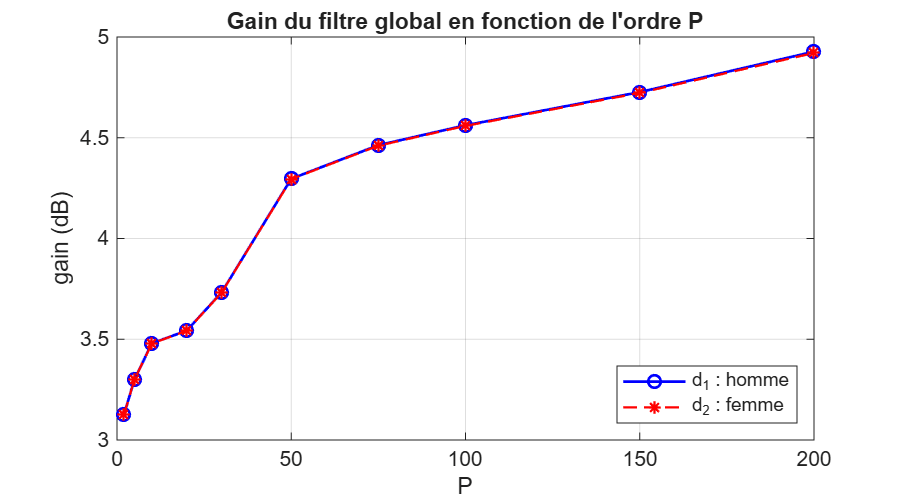
\includegraphics[width=\linewidth]{p4_q2_gain_P}
  \caption{Gain du filtre global en fonction de l'ordre $P$ (les deux courbes sont superposées).}
\end{figure}

\begin{figure}[H]
  \centering
  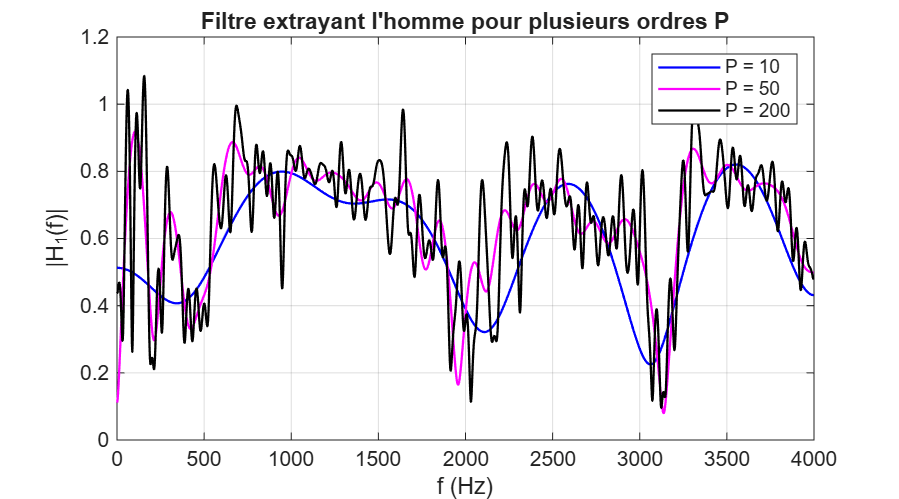
\includegraphics[width=\linewidth]{p4_q2_H1_P}
  \caption{Réponse en fréquence du filtre extrayant l'homme pour $P=10$, $50$ et $200$.}
\end{figure}

\begin{resultat}
Le gain passe de $3.13$~dB ($P=2$) à $3.48$~dB ($P=10$), $3.73$~dB ($P=30$), $\mathbf{4.30}$~dB ($P=50$) puis $4.93$~dB ($P=200$). Les gains des deux voix restent égaux à $0.01$~dB près.
\end{resultat}

\begin{interpretation}
\begin{itemize}
  \item \textbf{Un coude vers $P=50$.} Le saut le plus fort est entre $P=30$ et $P=50$ ($+0.57$~dB pour $20$ coefficients). Au-delà, le gain ne croît plus que lentement ($+0.63$~dB de $50$ à $200$, pour $150$ coefficients).
  \item \textbf{Lecture fréquentielle.} À $P=50$ ($\approx 160$~Hz de résolution), $H_1$ peut enfin suivre l'alternance des zones : $|H_1|\approx 0.9$ vers $100$--$150$~Hz (fondamental de l'homme), $\approx 0.3$ entre $200$ et $500$~Hz (zone de la femme), puis $0.7$--$0.9$ au-dessus. À $P=10$, cette zone était moyennée ($|H_1|\approx 0.4$--$0.5$).
  \item \textbf{Lecture temporelle.} La période fondamentale de la femme vaut $\approx F_s/200 = 40$ échantillons. Avec $P\geq 40$, le filtre couvre une période entière et exploite la périodicité de sa voix. C'est la même condition que $F_s/P\leq F_0$ : résoudre le fondamental en fréquence revient à couvrir une période en temps.
  \item \textbf{Au-delà de $P=50$.} $H_1$ devient très irrégulier à $P=200$ (variations de $0.1$ à $1.08$ sur quelques dizaines de Hz) : il suit les détails fins du spectre moyen. Ces détails sont en partie brouillés, car la hauteur des voix varie sur $8$~s, d'où un gain faible par coefficient ajouté.
  \item \textbf{Comparaison avec la partie~3.} Le coude y était à $P=10$ : contre un bruit blanc, une forme large suffisait. Ici, les deux spectres s'entrecroisent sur quelques centaines de Hz, ce qui demande un filtre plus fin.
\end{itemize}
\end{interpretation}

\begin{resultat}[Conclusion]
$P=50$ est le meilleur compromis pour le filtre global : il résout le fondamental des voix et donne l'essentiel du gain. Même à $P=200$, le gain reste limité ($<5$~dB) : le filtre global ne voit que les spectres moyens. Pour aller plus loin, il faut suivre l'évolution des spectres dans le temps, donc traiter par trames.
\end{resultat}

\subsection{Traitement par trames : longueur de trame et ordre}

\begin{enonce}
\textbf{Objectif :} Recalculer un filtre de Wiener sur chaque trame pour suivre la non-stationnarité de la parole. Sur $20$~ms, les spectres des deux voix diffèrent beaucoup plus qu'en moyenne : souvent, une voix se tait, les deux voix prononcent des sons différents, et la hauteur de chaque voix est stable.
\end{enonce}

\textbf{Le compromis.} L'estimateur biaisé $\hat r(k)=\frac1L\sum_n x(n)x(n-k)$ ne dispose que de $L-k$ produits. Pour une trame de $L=160$ échantillons ($20$~ms), $\hat r(0)$ utilise $160$ produits mais $\hat r(99)$ seulement $61$ (et il est biaisé d'un facteur $61/160$). Une trame courte suit mieux l'évolution des voix, mais impose un ordre $P$ petit devant $L$. Une trame longue estime bien les corrélations, mais revient vers les spectres moyens. Les cas $P>L/2$ ne sont pas calculés.

\textbf{Démarche.} Pour chaque trame (sans recouvrement), $\mathbf{w}_i$ est calculé à partir de $\hat r_x$ et $\hat r_{d_j}$ estimés sur la trame. Comme en partie~3, on utilise le signal propre de chaque trame : c'est le meilleur cas possible, le cas où $\mathbf{r}_{d_1}$ est inconnu est traité plus loin. Chaque trame est filtrée avec les $P-1$ échantillons précédents de $x$, pour que le filtre ne reparte pas d'une mémoire vide. Le gain est calculé sur le signal reconstruit entier. Pour $L=20$~ms et $P=20$, on calcule aussi le RSB avant et le gain de chaque trame où l'homme parle (puissance supérieure à $1$~\% de sa puissance moyenne).

\textbf{Code.} Filtrage par trames :
\begin{lstlisting}
function dhat = separation_trames(x, d, P, L)
% Filtre de Wiener recalcule sur chaque trame de L echantillons (sans recouvrement)
x = x(:); d = d(:);
N = length(x);
K = floor(N / L);                    % nombre de trames
dhat = zeros(N,1);

for i = 1:K
    idx = (i-1)*L+1 : i*L;           % indices de la trame i
    rx = xcorr(x(idx), P-1, 'biased'); rx = rx(P:end);
    rd = xcorr(d(idx), P-1, 'biased'); rd = rd(P:end);
    w  = toeplitz(rx) \ rd;          % filtre de la trame i

    % On filtre avec les P-1 echantillons passes de x (pas de remise a zero)
    deb = max(1, idx(1)-P+1);
    y = filter(w, 1, x(deb:idx(end)));
    dhat(idx) = y(end-L+1:end);
end
end
\end{lstlisting}

Script (extrait) :
\begin{lstlisting}
[d1, d2, x, Fs] = charger_voix(8);
gain = @(d, dh) 10*log10(mean(d.^2) / mean((d - dh).^2));   % RSB_av = 0 dB

%% Gain en fonction de la longueur de trame, pour plusieurs P
Lms   = [5 10 20 40 100 200];        % longueurs de trame (ms)
Plist = [10 20 50];
G1 = nan(length(Plist), length(Lms));  G2 = G1;
for p = 1:length(Plist)
    P = Plist(p);
    for l = 1:length(Lms)
        L = round(Lms(l)*1e-3*Fs);
        if P > L/2, continue; end    % trop peu d'echantillons pour estimer P retards
        G1(p,l) = gain(d1, separation_trames(x, d1, P, L));
        G2(p,l) = gain(d2, separation_trames(x, d2, P, L));
    end
end

%% Criteres par trame (L = 20 ms, P = 20)
P = 20;  L = round(20e-3*Fs);  K = floor(length(x)/L);
d1h = separation_trames(x, d1, P, L);
RSBav = nan(K,1);  g = nan(K,1);
for i = 1:K
    idx = (i-1)*L+1 : i*L;
    p1 = mean(d1(idx).^2);  p2 = mean(d2(idx).^2);
    if p1 < 0.01*mean(d1.^2), continue; end    % homme silencieux : trame ignoree
    RSBav(i) = 10*log10(p1 / p2);
    g(i)     = 10*log10(p1 / mean((d1(idx) - d1h(idx)).^2)) - RSBav(i);
end
\end{lstlisting}

\begin{figure}[H]
  \centering
  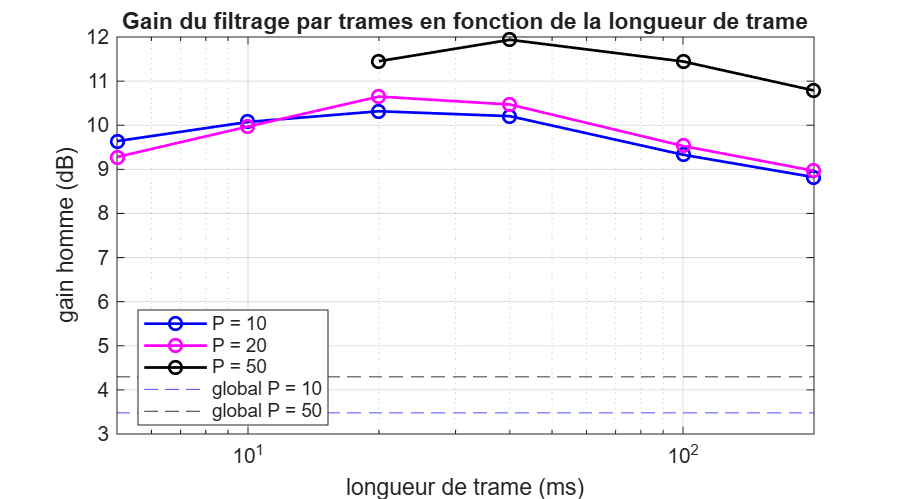
\includegraphics[width=\linewidth]{p4_q3_gain_L}
  \caption{Gain (homme) du filtrage par trames en fonction de la longueur de trame, pour $P=10$, $20$ et $50$. En pointillés : filtre global.}
\end{figure}

\begin{table}[H]
\centering
\small
\begin{tabular}{lcccccc}
\toprule
$L$ (ms) & 5 & 10 & 20 & 40 & 100 & 200 \\
\midrule
$P=10$ & 9.64 & 10.07 & \textbf{10.32} & 10.21 & 9.33 & 8.82 \\
$P=20$ & 9.28 & 9.97 & \textbf{10.65} & 10.47 & 9.53 & 8.97 \\
$P=50$ & -- & -- & 11.45 & \textbf{11.94} & 11.45 & 10.79 \\
\midrule
Global & \multicolumn{6}{c}{$3.48$~dB ($P=10$), $4.30$~dB ($P=50$)} \\
\bottomrule
\end{tabular}
\caption{Gain (dB) de l'homme selon $L$ et $P$. Les gains de la femme sont égaux à $0.6$~dB près.}
\end{table}

\begin{figure}[H]
  \centering
  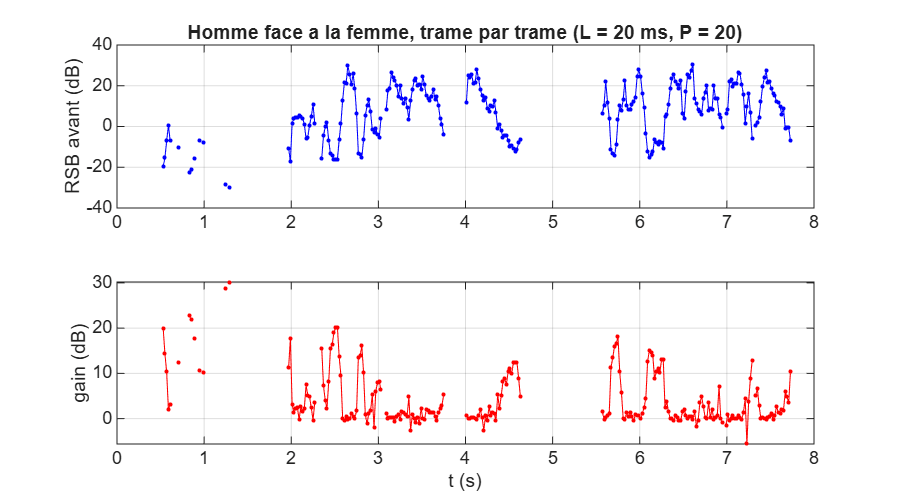
\includegraphics[width=\linewidth]{p4_q3_par_trame}
  \caption{RSB avant (homme face à la femme) et gain de chaque trame où l'homme parle ($L=20$~ms, $P=20$).}
\end{figure}

\begin{figure}[H]
  \centering
  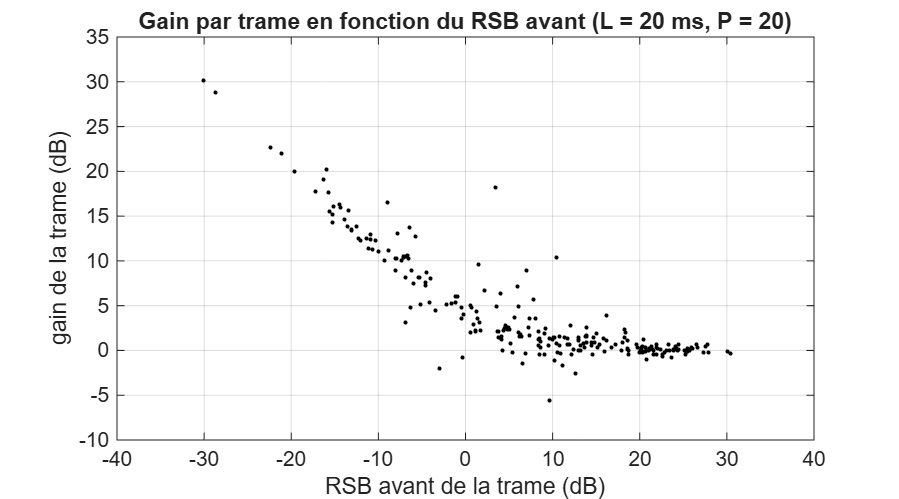
\includegraphics[width=0.85\linewidth]{p4_q3_gain_vs_RSB}
  \caption{Gain de chaque trame en fonction de son RSB avant ($L=20$~ms, $P=20$).}
\end{figure}

\begin{resultat}
Le gain passe de $4.30$~dB (global, $P=50$) à $\mathbf{11.94}$~dB (trames de $40$~ms, $P=50$), soit $+7.6$~dB. À l'écoute, chaque estimée ne contient presque plus que la voix recherchée. Gain moyen par trame ($L=20$~ms, $P=20$, trames où l'homme parle) : $4.29$~dB.
\end{resultat}

\begin{interpretation}
\begin{itemize}
  \item \textbf{Optimum de longueur de trame.} Chaque courbe a un maximum entre $20$ et $40$~ms. Pour des trames courtes, l'estimation des corrélations est bruitée : à $5$~ms ($40$ échantillons), $P=20$ ($=L/2$) fait moins bien que $P=10$. Pour des trames longues, on revient vers les spectres moyens : le gain baisse de $1$ à $1.5$~dB à $200$~ms. L'optimum se déplace vers des trames plus longues quand $P$ augmente ($20$~ms pour $P=10$ et $20$, $40$~ms pour $P=50$) : plus de retards à estimer demande plus d'échantillons.
  \item \textbf{D'où vient le gain.} Trame par trame, le RSB avant varie de $-30$ à $+30$~dB : la plupart du temps, une voix domine nettement. Le filtre se comporte alors presque comme un interrupteur, $\mathbf{w}_i\approx[1,0,\dots,0]^T$ (laisser passer) si la cible domine, $\mathbf{w}_i\approx\mathbf{0}$ (couper) sinon. Même avec $P=10$, dont la résolution en fréquence est grossière, le gain atteint $10$~dB : l'essentiel de la séparation vient de la sélection dans le temps, pas de la forme du spectre.
  \item \textbf{Gain par trame et RSB avant.} Quand l'homme est noyé (RSB avant $<0$), le gain vaut presque $-\mathrm{RSB}_{\mathrm{av}}$ : le filtre coupe la trame, donc $\hat d_1\approx 0$, l'erreur vaut $d_1$ et le RSB après vaut $\approx 0$~dB. La femme est supprimée, mais l'homme n'est pas récupéré. Quand l'homme domine ($>20$~dB), le gain est nul : le filtre laisse tout passer. La vraie séparation spectrale n'a lieu qu'entre $0$ et $10$~dB, avec quelques dB de gain.
  \item \textbf{Gain moyen par trame ($4.29$~dB) et gain global ($10.65$~dB).} La moyenne des gains en dB donne le même poids à chaque trame, et beaucoup de trames où l'homme domine ont un gain proche de $0$. Le gain global compare des énergies totales : il compte aussi les trames où l'homme se tait, que le filtre coupe presque parfaitement, alors que le filtre global laissait passer la femme pendant ces silences. Les deux critères mesurent des choses différentes.
  \item \textbf{Limite.} Ce résultat suppose $\mathbf{r}_{d_1}$ connu sur chaque trame, c'est-à-dire qu'on sait à chaque instant qui parle et avec quel spectre. C'est une borne supérieure ; le cas réaliste est traité dans les sections sur la robustesse.
\end{itemize}
\end{interpretation}

\begin{resultat}[Conclusion]
Le traitement par trames est l'étape décisive : il fait passer le gain d'environ $4$~dB à $10$--$12$~dB, et la séparation devient nette à l'écoute. Le meilleur réglage est une trame de $20$ à $40$~ms avec $P$ petit devant $L$ ($P=50$ et $L=40$~ms ici). Ce gain vient surtout de ce que, sur une trame courte, une voix domine presque toujours l'autre.
\end{resultat}

%==================== CONCLUSION ====================
\section{Conclusion}

Ce TP a mis en œuvre le filtre de Wiener sur une sinusoïde bruitée puis sur un signal audio réel. Le filtre est obtenu en résolvant $\mathbf{R}_x\mathbf{w}_{opt}=\mathbf{r}_{dx}$, et l'erreur minimale $\mathrm{EQM}_{\min}=r_d(0)-\mathbf{w}_{opt}^T\mathbf{r}_{dx}$ correspond à l'erreur observée en simulation, à une erreur d'estimation près qui diminue quand $N$ augmente.

\begin{interpretation}[Ce qu'il faut retenir]
\begin{itemize}
  \item \textbf{Ordre du filtre.} $\mathrm{EQM}_{\min}$ diminue avec $P$ puis atteint un palier : $P\approx 25$ pour la sinusoïde ($\approx 11$~dB de gain), $P=10$ pour le signal audio, dont la corrélation décroît rapidement.
  \item \textbf{Débruitage par trames.} Il suit mieux la non-stationnarité du signal audio, mais n'améliore le gain du signal reconstruit que de $\approx 0.2$~dB et crée des clics aux frontières : des trames de $20$ à $50$~ms sont un meilleur compromis que $3$~ms.
  \item \textbf{Limites du critère.} Le gain en RSB augmente mécaniquement quand le bruit domine et ne mesure ni les discontinuités ni le bruit résiduel audible.
  \item \textbf{Limites du filtre.} Il suppose des statistiques connues et un signal stationnaire. Sans signal propre, $r_d(k)$ doit être estimé sur le signal bruité (trames longues nécessaires), et un bruit coloré dans la bande du signal ne peut pas être éliminé.
\end{itemize}
\end{interpretation}

Ces limites justifient l'approche de Widrow (partie~1) : le LMS ajuste les coefficients à chaque échantillon, sans connaître les statistiques et sans découpage en trames. Le comparer au filtre de Wiener sur le même signal audio serait une suite naturelle de ce travail.

\begin{thebibliography}{10}
\addcontentsline{toc}{section}{Références}
\bibitem{wiener1949} N.~Wiener, \emph{Extrapolation, Interpolation, and Smoothing of Stationary Time Series}, MIT Press / Wiley, 1949.
\bibitem{wiener1948} N.~Wiener, \emph{Cybernetics: or Control and Communication in the Animal and the Machine}, MIT Press / Wiley, 1948.
\bibitem{ethw_wiener} ETHW, « Norbert Wiener », \url{https://ethw.org/Norbert_Wiener}.
\bibitem{wiki_wiener} Wikipedia, « Norbert Wiener », \url{https://en.wikipedia.org/wiki/Norbert_Wiener}.
\bibitem{monoskop} Monoskop, « Norbert Wiener », \url{https://monoskop.org/Norbert_Wiener}.
\bibitem{ethw_widrow} ETHW, « Bernard Widrow », \url{https://ethw.org/Bernard_Widrow}.
\bibitem{chm_widrow} Computer History Museum, « Widrow, Bernard oral history », \url{https://www.computerhistory.org/collections/catalog/102746758}.
\bibitem{stanford_obit} Stanford Magazine, « Trailblazer of Computers that Learn », \url{https://stanfordmag.org/contents/trailblazer-of-computers-that-learn}.
\bibitem{widrowstearns} B.~Widrow et S.~D.~Stearns, \emph{Adaptive Signal Processing}, Prentice-Hall, 1985.
\bibitem{osr} Open Speech Repository, « American English », \url{https://www.voiptroubleshooter.com/open_speech/american.html}.
\bibitem{widrowlehr1990} B.~Widrow et M.~A.~Lehr, « 30 Years of Adaptive Neural Networks: Perceptron, Madaline, and Backpropagation », \emph{Proc. IEEE}, vol.~78, n°~9, pp.~1415--1442, 1990.
\end{thebibliography}
\end{document}
